\documentclass[aspectratio=169]{beamer}\usepackage[]{graphicx}\usepackage[]{xcolor}
% maxwidth is the original width if it is less than linewidth
% otherwise use linewidth (to make sure the graphics do not exceed the margin)
\makeatletter
\def\maxwidth{ %
  \ifdim\Gin@nat@width>\linewidth
    \linewidth
  \else
    \Gin@nat@width
  \fi
}
\makeatother

\definecolor{fgcolor}{rgb}{0.345, 0.345, 0.345}
\newcommand{\hlnum}[1]{\textcolor[rgb]{0.686,0.059,0.569}{#1}}%
\newcommand{\hlsng}[1]{\textcolor[rgb]{0.192,0.494,0.8}{#1}}%
\newcommand{\hlcom}[1]{\textcolor[rgb]{0.678,0.584,0.686}{\textit{#1}}}%
\newcommand{\hlopt}[1]{\textcolor[rgb]{0,0,0}{#1}}%
\newcommand{\hldef}[1]{\textcolor[rgb]{0.345,0.345,0.345}{#1}}%
\newcommand{\hlkwa}[1]{\textcolor[rgb]{0.161,0.373,0.58}{\textbf{#1}}}%
\newcommand{\hlkwb}[1]{\textcolor[rgb]{0.69,0.353,0.396}{#1}}%
\newcommand{\hlkwc}[1]{\textcolor[rgb]{0.333,0.667,0.333}{#1}}%
\newcommand{\hlkwd}[1]{\textcolor[rgb]{0.737,0.353,0.396}{\textbf{#1}}}%
\let\hlipl\hlkwb

\usepackage{framed}
\makeatletter
\newenvironment{kframe}{%
 \def\at@end@of@kframe{}%
 \ifinner\ifhmode%
  \def\at@end@of@kframe{\end{minipage}}%
  \begin{minipage}{\columnwidth}%
 \fi\fi%
 \def\FrameCommand##1{\hskip\@totalleftmargin \hskip-\fboxsep
 \colorbox{shadecolor}{##1}\hskip-\fboxsep
     % There is no \\@totalrightmargin, so:
     \hskip-\linewidth \hskip-\@totalleftmargin \hskip\columnwidth}%
 \MakeFramed {\advance\hsize-\width
   \@totalleftmargin\z@ \linewidth\hsize
   \@setminipage}}%
 {\par\unskip\endMakeFramed%
 \at@end@of@kframe}
\makeatother

\definecolor{shadecolor}{rgb}{.97, .97, .97}
\definecolor{messagecolor}{rgb}{0, 0, 0}
\definecolor{warningcolor}{rgb}{1, 0, 1}
\definecolor{errorcolor}{rgb}{1, 0, 0}
\newenvironment{knitrout}{}{} % an empty environment to be redefined in TeX

\usepackage{alltt}

% Set lecture number for later use


% Part common to all the lectures
\subtitle{MATH 2740 -- Mathematics of Data Science -- Lecture 15}
\author{\texorpdfstring{Julien Arino\newline\url{julien.arino@umanitoba.ca}}{Julien Arino}}
\institute{Department of Mathematics @ University of Manitoba}
\date{Fall 202X}

% Title of the lecture
\title{Graphs -- Introduction (theory) -- 1}



\usetheme{default}
% Slide setup, colour independent

\usepackage{amsmath,amssymb,amsthm}
\usepackage[utf8]{inputenc}
\usepackage{colortbl}
\usepackage{bm}
\usepackage{xcolor}
\usepackage{dsfont}
\usepackage{setspace}
% To use \ding{234} and the like
\usepackage{pifont}
% To cross reference between slide files
\usepackage{zref-xr,zref-user}
% Use something like
% \zexternaldocument{fileI}
% in the tex files. And cite using \zref instead of \ref

% Cross-reference system - see CROSS-REFERENCE-SETUP.md for manual setup instructions
\usepackage{booktabs}
\usepackage{marvosym}
\usepackage{cancel}
%\usepackage{transparent}
% Make doi clickable in the bibliography?
\usepackage{doi}

\usepackage[T1]{fontenc}

\usepackage{longtable}

% For heavier titles
\usepackage{helvet} % Enables Helvetica font family


% Fields and the like
\def\IC{\mathbb{C}}
\def\IE{\mathbb{E}}
\def\IF{\mathbb{F}}
\def\II{\mathbb{I}}
\def\IJ{\mathbb{J}}
\def\IK{\mathbb{K}}
\def\IM{\mathbb{M}}
\def\IN{\mathbb{N}}
\def\IP{\mathbb{P}}
\def\IR{\mathbb{R}}
\newcommand{\IRplus}{\mathbb{R}_{\ge 0}}
\def\IZ{\mathbb{Z}}
\def\11{\mathds{1}}


% Bold lowercase
\def\ba{\bm{a}}
\def\bb{\bm{b}}
\def\bc{\bm{c}}
\def\bd{\bm{d}}
\def\be{\bm{e}}
\def\bf{\bm{f}}
\def\bg{\bm{g}}
\def\bh{\bm{h}}
\def\bi{\bm{i}}
\def\bj{\bm{j}}
\def\bk{\bm{k}}
\def\bn{\bm{n}}
\def\bp{\bm{p}}
\def\br{\bm{r}}
\def\bs{\bm{s}}
\def\bu{\bm{u}}
\def\bv{\bm{v}}
\def\bw{\bm{w}}
\def\bx{\bm{x}}
\def\by{\bm{y}}
\def\bz{\bm{z}}
\newcommand{\vect}[1]{\bm{#1}}

% Bold capitals
\def\bB{\bm{B}}
\def\bD{\bm{D}}
\def\bE{\bm{E}}
\def\bF{\bm{F}}
\def\bG{\bm{G}}
\def\bI{\bm{I}}
\def\bL{\bm{L}}
\def\bN{\bm{N}}
\def\bP{\bm{P}}
\def\bR{\bm{R}}
\def\bS{\bm{S}}
\def\bT{\bm{T}}
\def\bX{\bm{X}}

% Bold numbers
\def\b0{\bm{0}}

% Bold greek
\bmdefine{\bmu}{\bm{\mu}}
\def\bphi{\bm{\phi}}
\def\bvarphi{\bm{\varphi}}
\def\bPi{\bm{\Pi}}
\def\bGamma{\bm{\Gamma}}

% Bold red sentence
\def\boldred#1{{\color{red}\textbf{#1}}}
\def\defword#1{{\color{orange}\textbf{#1}}}

% Caligraphic letters
\def\A{\mathcal{A}}
\def\B{\mathcal{B}}
\def\C{\mathcal{C}}
\def\D{\mathcal{D}}
\def\E{\mathcal{E}}
\def\F{\mathcal{F}}
\def\G{\mathcal{G}}
\def\H{\mathcal{H}}
\def\I{\mathcal{I}}
\def\L{\mathcal{L}}
\def\M{\mathcal{M}}
\def\N{\mathcal{N}}
\def\P{\mathcal{P}}
\def\R{\mathcal{R}}
\def\S{\mathcal{S}}
\def\T{\mathcal{T}}
\def\U{\mathcal{U}}
\def\V{\mathcal{V}}

% Adding space for prime (') where needed
\def\pprime{\,'}
% Adding space for star (\star) where needed
\def\pstar{{\,\star}}

% tt font for code
\def\code#1{{\tt #1}}

% i.e., e.g.
\def\eg{\emph{e.g.}}
\def\ie{\emph{i.e.}}


% Operators and special symbols
\def\nbOne{{\mathchoice {\rm 1\mskip-4mu l} {\rm 1\mskip-4mu l}
{\rm 1\mskip-4.5mu l} {\rm 1\mskip-5mu l}}}
\def\cov{\ensuremath{\mathsf{cov}}}
\def\Var{\ensuremath{\mathsf{Var}\ }}
\def\Im{\textrm{Im}\;}
\def\Re{\textrm{Re}\;}
\def\det{\ensuremath{\mathsf{det}}}
\def\diag{\ensuremath{\mathsf{diag}}}
\def\nullspace{\ensuremath{\mathsf{null}}}
\def\nullity{\ensuremath{\mathsf{nullity}}}
\def\rank{\ensuremath{\mathsf{rank}}}
\def\range{\ensuremath{\mathsf{range}}}
\def\sgn{\ensuremath{\mathsf{sgn}}}
\def\Span{\ensuremath{\mathsf{span}}}
\def\tr{\ensuremath{\mathsf{tr}}}
\def\imply{$\Rightarrow$}
\def\restrictTo#1#2{\left.#1\right|_{#2}}
\newcommand{\parallelsum}{\mathbin{\!/\mkern-5mu/\!}}
\def\dsum{\mathop{\displaystyle \sum }}%
\def\dind#1#2{_{\substack{#1\\ #2}}}

\newcommand{\Qmatrix}[1]{%
  \begin{pmatrix}#1\end{pmatrix}%
}

\DeclareMathOperator{\GL}{GL}
\DeclareMathOperator{\Rel}{Re}
\def\Nt#1{\left|\!\left|\!\left|#1\right|\!\right|\!\right|}
\newcommand{\tripbar}{|\! |\! |}



% The beamer bullet (in base colour)
\def\bbullet{\leavevmode\usebeamertemplate{itemize item}\ }

% Theorems and the like
\newtheorem{proposition}[theorem]{Proposition}
\newtheorem{property}[theorem]{Property}
\newtheorem{importantproperty}[theorem]{Property}
\newtheorem{importanttheorem}[theorem]{Theorem}
%\newtheorem{lemma}[theorem]{Lemma}
%\newtheorem{corollary}[theorem]{Corollary}
\newtheorem{remark}[theorem]{Remark}
\setbeamertemplate{theorems}[numbered]
%\setbeamertemplate{theorems}[ams style]

%
%\usecolortheme{orchid}
%\usecolortheme{orchid}

\def\red{\color[rgb]{1,0,0}}
\def\blue{\color[rgb]{0,0,1}}
\def\green{\color[rgb]{0,1,0}}

% Fix skipping lines after items in the bibliography
\setbeamertemplate{bibliography entry title}{}
\setbeamertemplate{bibliography entry location}{}
\setbeamertemplate{bibliography entry note}{}

% Get rid of navigation stuff
\setbeamertemplate{navigation symbols}{}

% Set footline/header line
\setbeamertemplate{footline}
{%
\quad p. \insertpagenumber \quad--\quad \insertsection\vskip2pt
}
% \setbeamertemplate{headline}
% {%
% \quad\insertsection\hfill p. \insertpagenumber\quad\mbox{}\vskip2pt
% }


\makeatletter
\newlength\beamerleftmargin
\setlength\beamerleftmargin{\Gm@lmargin}
\makeatother

% Colours for special pages
\def\extraContent{yellow!20}


%%%%%%%%%%%%%%%%%
\usepackage{tikz}
\usetikzlibrary{shapes,arrows}
\usetikzlibrary{positioning}
\usetikzlibrary{shapes.symbols,shapes.callouts,patterns}
\usetikzlibrary{calc,fit}
\usetikzlibrary{backgrounds}
\usetikzlibrary{decorations.pathmorphing,fit,petri}
\usetikzlibrary{automata}
\usetikzlibrary{fadings}
\usetikzlibrary{patterns,hobby}
\usetikzlibrary{backgrounds,fit,petri}
\usetikzlibrary{tikzmark}

\usepackage{pgfplots}
\pgfplotsset{compat=1.6}
\pgfplotsset{ticks=none}

\usetikzlibrary{decorations.markings}
\usetikzlibrary{arrows.meta}
\tikzset{>=stealth}

% For tikz
\tikzstyle{cloud} = [draw, ellipse,fill=red!20, node distance=0.87cm,
minimum height=2em]
\tikzstyle{line} = [draw, -latex']


%%% For max frame images
\newenvironment{changemargin}[2]{%
\begin{list}{}{%
\setlength{\topsep}{0pt}%
\setlength{\leftmargin}{#1}%
\setlength{\rightmargin}{#2}%
\setlength{\listparindent}{\parindent}%
\setlength{\itemindent}{\parindent}%
\setlength{\parsep}{\parskip}%
}%
\item[]}{\end{list}}


% Make one image take up the entire slide content area in beamer,.:
% centered/centred full-screen image, with title:
% This uses the whole screen except for the 1cm border around it
% all. 128x96mm
\newcommand{\titledFrameImage}[2]{
\begin{frame}{#1}
%\begin{changemargin}{-1cm}{-1cm}
\begin{center}
\includegraphics[width=108mm,height=\textheight,keepaspectratio]{#2}
\end{center}
%\end{changemargin}
\end{frame}
}

% Make one image take up the entire slide content area in beamer.:
% centered/centred full-screen image, no title:
% This uses the whole screen except for the 1cm border around it
% all. 128x96mm
\newcommand{\plainFrameImage}[1]{
\begin{frame}[plain]
%\begin{changemargin}{-1cm}{-1cm}
\begin{center}
\includegraphics[width=108mm,height=76mm,keepaspectratio]{#1}
\end{center}
%\end{changemargin}
\end{frame}
}

% Make one image take up the entire slide area, including borders, in beamer.:
% centered/centred full-screen image, no title:
% This uses the entire whole screen
\newcommand{\maxFrameImage}[1]{
\begin{frame}[plain]
\begin{changemargin}{-1cm}{-1cm}
\begin{center}
\includegraphics[width=\paperwidth,height=\paperheight,keepaspectratio]
{#1}
\end{center}
\end{changemargin}
\end{frame}
}

% This uses the entire whole screen (to include in frame)
\newcommand{\maxFrameImageNoFrame}[1]{
\begin{changemargin}{-1cm}{-1cm}
\begin{center}
\includegraphics[width=\paperwidth,height=0.99\paperheight,keepaspectratio]
{#1}
\end{center}
\end{changemargin}
}

% Make one image take up the entire slide area, including borders, in beamer.:
% centered/centred full-screen image, no title:
% This uses the entire whole screen
\newcommand{\maxFrameImageColor}[2]{
\begin{frame}[plain]
\setbeamercolor{normal text}{bg=#2!20}
\begin{changemargin}{-1cm}{-1cm}
\begin{center}
\includegraphics[width=\paperwidth,height=\paperheight,keepaspectratio]
{#1}
\end{center}
\end{changemargin}
\end{frame}
}


\usepackage{tikz}
\usetikzlibrary{patterns,hobby,matrix}
\usepackage{pgfplots}
\pgfplotsset{compat=1.6}
\pgfplotsset{ticks=none}

\usetikzlibrary{backgrounds}
\usetikzlibrary{decorations.markings}
\usetikzlibrary{arrows.meta}
\tikzset{>=stealth}

\tikzset{
  clockwise arrows/.style={
    postaction={
      decorate,
      decoration={
        markings,
        mark=between positions 0.1 and 0.9 step 40pt with {\arrow{>}},
   }}}}


% New integrated section command: creates section and section slide
\newcommand{\Ssection}[2]{
\section{#1}
\begin{frame}[noframenumbering,plain]
  \begin{tikzpicture}[remember picture,overlay]
    \node[above right,inner sep=0pt,opacity=0.2] at (current page.south west)
    {
        \includegraphics[height=\paperheight,width=\paperwidth]{#2}
    };
  \end{tikzpicture}
  \setbeamercolor{section in toc}{fg=section_page_list_colour}
  \setbeamerfont{section in toc}{size=\Large,series=\bfseries}
  \setbeamertemplate{section in toc shaded}[default][60]
  \tableofcontents[
    currentsection,
    sectionstyle=show/shaded,
    subsectionstyle=show/hide/hide,
    subsubsectionstyle=hide/hide/hide]
\end{frame}
\addtocounter{page}{-1}
}

% New integrated section command with subsections: creates section and section slide showing subsections
\newcommand{\SsectionWithSubs}[2]{
\section{#1}
\begin{frame}[noframenumbering,plain]
  \begin{tikzpicture}[remember picture,overlay]
    \node[above right,inner sep=0pt,opacity=0.2] at (current page.south west)
    {
        \includegraphics[height=\paperheight,width=\paperwidth]{#2}
    };
  \end{tikzpicture}
  \setbeamercolor{section in toc}{fg=section_page_list_colour}
  \setbeamerfont{section in toc}{size=\Large,series=\bfseries}
  \setbeamertemplate{section in toc shaded}[default][60]
  \tableofcontents[
    currentsection,
    sectionstyle=show/hide,
    subsectionstyle=show/show/hide,
    subsubsectionstyle=hide/hide/hide]
\end{frame}
\addtocounter{page}{-1}
}

% New integrated subsection command: creates subsection and subsection slide
\newcommand{\Ssubsection}[2]{
\subsection{#1}
\begin{frame}[noframenumbering,plain]
  \begin{tikzpicture}[remember picture,overlay]
    \node[above right,inner sep=0pt,opacity=0.2] at (current page.south west)
    {
        \includegraphics[height=\paperheight,width=\paperwidth]{#2}
    };
  \end{tikzpicture}
  \setbeamercolor{section in toc}{fg=subsection_page_list_colour}
  \setbeamerfont{section in toc}{size=\Large,series=\bfseries}
  \setbeamertemplate{section in toc shaded}[default][60]
  \setbeamerfont{subsection in toc}{series=\bfseries}
  \setbeamertemplate{subsection in toc shaded}[default][50]
  \tableofcontents[
    currentsection,
    sectionstyle=show/hide,
    subsectionstyle=show/shaded/hide,
    subsubsectionstyle=hide/hide/hide]
\end{frame}
\addtocounter{page}{-1}
}

% New integrated subsubsection command: creates subsubsection and subsubsection slide
\newcommand{\Ssubsubsection}[2]{
\subsubsection{#1}
\begin{frame}[noframenumbering,plain]
  \begin{tikzpicture}[remember picture,overlay]
    \node[above right,inner sep=0pt,opacity=0.2] at (current page.south west)
    {
        \includegraphics[height=\paperheight,width=\paperwidth]{#2}
    };
  \end{tikzpicture}
  \setbeamercolor{section in toc}{fg=subsub_header_section}
  \setbeamerfont{section in toc}{size=\Large,series=\bfseries}
  \setbeamertemplate{section in toc shaded}[default][60]
  \setbeamerfont{subsection in toc}{series=\bfseries}
  \setbeamertemplate{subsection in toc shaded}[default][50]
  \setbeamertemplate{subsubsection in toc shaded}[default][50]
  \tableofcontents[
    currentsection,
    sectionstyle=show/hide,
    subsectionstyle=show/hide/hide,
    subsubsectionstyle=show/shaded/hide]
\end{frame}
\addtocounter{page}{-1}
}

% Legacy commands (kept for backward compatibility)
% Beginning of a section
\newcommand{\newSectionSlide}[1]{
\begin{frame}[noframenumbering,plain]
  \begin{tikzpicture}[remember picture,overlay]
    \node[above right,inner sep=0pt,opacity=0.2] at (current page.south west)
    {
        \includegraphics[height=\paperheight,width=\paperwidth]{#1}
    };
  \end{tikzpicture}
  \setbeamercolor{section in toc}{fg=section_page_list_colour}
  \setbeamerfont{section in toc}{size=\Large,series=\bfseries}
  \setbeamertemplate{section in toc shaded}[default][60]
  \tableofcontents[
    currentsection,
    sectionstyle=show/shaded,
    subsectionstyle=show/hide/hide,
    subsubsectionstyle=hide/hide/hide]
\end{frame}
\addtocounter{page}{-1}
}

% Beginning of a section in which we also show subsections
\newcommand{\newSectionWithSubsSlide}[1]{
	\begin{frame}[noframenumbering,plain]
		\begin{tikzpicture}[remember picture,overlay]
			\node[above right,inner sep=0pt,opacity=0.2] at (current page.south west)
			{
				\includegraphics[height=\paperheight,width=\paperwidth]{#1}
			};
		\end{tikzpicture}
		\setbeamercolor{section in toc}{fg=section_page_list_colour}
		\setbeamerfont{section in toc}{size=\Large,series=\bfseries}
		\setbeamertemplate{section in toc shaded}[default][60]
		\tableofcontents[
		currentsection,
		sectionstyle=show/hide,
		subsectionstyle=show/show/hide,
		subsubsectionstyle=hide/hide/hide]
	\end{frame}
	\addtocounter{page}{-1}
}

% Beginning of a subsection
\newcommand{\newSubSectionSlide}[1]{
\begin{frame}[noframenumbering,plain]
  \begin{tikzpicture}[remember picture,overlay]
    \node[above right,inner sep=0pt,opacity=0.2] at (current page.south west)
    {
        \includegraphics[height=\paperheight,width=\paperwidth]{#1}
    };
  \end{tikzpicture}
  \setbeamercolor{section in toc}{fg=subsection_page_list_colour}
  \setbeamerfont{section in toc}{size=\Large,series=\bfseries}
  \setbeamertemplate{section in toc shaded}[default][60]
  \setbeamerfont{subsection in toc}{series=\bfseries}
  \setbeamertemplate{subsection in toc shaded}[default][50]
  \tableofcontents[
    currentsection,
    sectionstyle=show/hide,
    subsectionstyle=show/shaded/hide,
    subsubsectionstyle=hide/hide/hide]
\end{frame}
\addtocounter{page}{-1}
}

% Beginning of a subsubsection
\newcommand{\newSubSubSectionSlide}[1]{
\begin{frame}[noframenumbering,plain]
  \begin{tikzpicture}[remember picture,overlay]
    \node[above right,inner sep=0pt,opacity=0.2] at (current page.south west)
    {
        \includegraphics[height=\paperheight,width=\paperwidth]{#1}
    };
  \end{tikzpicture}
  \setbeamercolor{section in toc}{fg=subsub_header_section}
  \setbeamerfont{section in toc}{size=\Large,series=\bfseries}
  \setbeamertemplate{section in toc shaded}[default][60]
  \setbeamerfont{subsection in toc}{series=\bfseries}
  \setbeamertemplate{subsection in toc shaded}[default][50]
  \setbeamertemplate{subsubsection in toc shaded}[default][50]
  \tableofcontents[
    currentsection,
    sectionstyle=show/hide,
    subsectionstyle=show/hide/hide,
    subsubsectionstyle=show/shaded/hide]
\end{frame}
\addtocounter{page}{-1}
}


   %%%%%%%%%%%
% To have links to parts in the outline
\makeatletter
\AtBeginPart{%
  \addtocontents{toc}{\protect\beamer@partintoc{\the\c@part}{\beamer@partnameshort}{\the\c@page}}%
}
%% number, shortname, page.
\providecommand\beamer@partintoc[3]{%
  \ifnum\c@tocdepth=-1\relax
    % requesting onlyparts.
    \makebox[6em]{Part #1:} \textcolor{green!30!blue}{\hyperlink{#2}{#2}}
    \par
  \fi
}
\define@key{beamertoc}{onlyparts}[]{%
  \c@tocdepth=-1\relax
}
\makeatother%

\newcommand{\nameofthepart}{}
\newcommand{\nupart}[1]%
    {   \part{#1}%
        \renewcommand{\nameofthepart}{#1}%
        {
          \setbeamercolor{background canvas}{bg=orange!50}
          \begin{frame}{#1}%\partpage 
          \hypertarget{\nameofthepart}{}\tableofcontents%
          \end{frame}
        }
    }

% This command creates a title page using TikZ only
\newcommand{\tikztitlepage}[1]{%
\begin{frame}[plain,noframenumbering]
  \begin{tikzpicture}[remember picture,overlay]
    % Background image
    \node[above right,inner sep=0pt,opacity=0.1] 
      at (current page.south west) 
      {\includegraphics[width=\paperwidth,height=\paperheight]{#1}};

    % University logo
    \node[anchor=north east, inner sep=5pt, opacity=0.9] 
      at (current page.north east)
      {
\includegraphics[width=0.2\textwidth]{FIGS-slides-admin/UM-logo-horizontal-CMYK.png}};
    
    % Title
    \node[anchor=center, align=center, 
          font=\fontsize{13}{15}\bfseries\color{UMbrown}, 
          text width=0.9\textwidth] 
          at ([yshift=2cm]current page.center)
          {\inserttitle};

      % Authors
      \node[anchor=center, align=center,
        font=\fontsize{10}{12}\bfseries\color{UMbrown},
        text width=0.7\textwidth]
        at ([yshift=0.8cm]current page.center)
        {\insertauthor};

      % Affiliation
      \node[anchor=north, align=center,
        font=\fontsize{9}{11}\color{UMbrown},
        text width=0.7\textwidth]
        at ([yshift=-0.2cm]current page.center)
        {\insertaffiliation};      
    % Date
    \node[anchor=north, align=center, 
          font=\fontsize{12}{16}\bfseries\color{UMbrown},
          text width=0.7\textwidth] 
          at ([yshift=0.2cm]current page.center)
          {\insertdate};

    % Land acknowledgement
    \node[anchor=south, align=justify, 
          font=\footnotesize, text=black, 
          text width=1.1\textwidth] 
          at ([yshift=0.5cm]current page.south)
          {The University of Manitoba campuses are located on original lands of Anishinaabeg, Ininew, Anisininew, Dakota and Dene peoples, and on the National Homeland of the Red River Métis.\\
          We respect the Treaties that were made on these territories, we acknowledge the harms and mistakes of the past, and we dedicate ourselves to move forward in partnership with Indigenous communities in a spirit of Reconciliation and collaboration.};
  \end{tikzpicture}
  \addtocounter{page}{-1}
\end{frame}
}
% The title page with figure
% \newcommand{\titlepagewithfigure}[1]{%
%   \begin{frame}[noframenumbering,plain]
%     \begin{tikzpicture}[remember picture,overlay]
%       \node[above right,inner sep=0pt,opacity=0.1] at (current page.south west)
%       {
%           \includegraphics[height=\paperheight,width=\paperwidth]{#1}
%       };
%       \node[anchor=north east,
%       inner sep=5pt,
%       opacity=0.9] at (current page.north east)
%       {
%           
\includegraphics[width=0.2\textwidth]{FIGS-slides-admin/UM-logo-horizontal-CMYK.png}
%       };
%       \node[anchor=south, 
%       align=justify, 
%       text=black, 
%       text width=1.1\textwidth,
%       font=\footnotesize]  (land_acknowledgement)
%       at (current page.south) 
%       {The University of Manitoba campuses are located on original lands of Anishinaabeg, Ininew, Anisininew, Dakota and Dene peoples, and on the National Homeland of the Red River Métis.
%       We respect the Treaties that were made on these territories, we acknowledge the harms and mistakes of the past, and we dedicate ourselves to move forward in partnership with Indigenous communities in a spirit of Reconciliation and collaboration.};  
%       % \node[align=center, anchor=south,
%       % above=0.5cm of land_acknowledgement,
%       % text=black,
%       % font=\bfseries] {\insertdate};
%   \end{tikzpicture}
%   \setbeamercolor{title}{fg=title_page_title_colour}
%   \setbeamerfont{title}{size=\Large,series=\bfseries}
%   \setbeamercolor{author}{fg=title_page_author_colour}
%   \setbeamerfont{author}{size=\large,series=\bfseries}
%   \setbeamercolor{institute}{fg=title_page_institute_colour}
%   \setbeamerfont{institute}{size=\large,series=\bfseries}
%   \setbeamercolor{date}{fg=title_page_date_colour}
%   \setbeamerfont{date}{series=\bfseries}
% 	\titlepage
% \end{frame}
% \addtocounter{page}{-1}
% }

\newcommand{\titlepagewithfigure}[1]{%
  \begin{frame}[noframenumbering,plain]
    \begin{tikzpicture}[remember picture,overlay]
      \node[above right,inner sep=0pt,opacity=0.1] at (current page.south west)
      {
          \includegraphics[height=\paperheight,width=\paperwidth]{#1}
      };
      \node[anchor=north east,
      inner sep=5pt,
      opacity=0.9] at (current page.north east)
      {
          
\includegraphics[width=0.2\textwidth]{FIGS-slides-admin/UM-logo-horizontal-CMYK.png}
      };
      \node[anchor=south, 
      align=justify, 
      text=black, 
      text width=1.1\textwidth,
      font=\footnotesize]  (land_acknowledgement)
      at (current page.south) 
      {The University of Manitoba campuses are located on original lands of Anishinaabeg, Ininew, Anisininew, Dakota and Dene peoples, and on the National Homeland of the Red River Métis.
      We respect the Treaties that were made on these territories, we acknowledge the harms and mistakes of the past, and we dedicate ourselves to move forward in partnership with Indigenous communities in a spirit of Reconciliation and collaboration.};  
      % \node[align=center, anchor=south,
      % above=0.5cm of land_acknowledgement,
      % text=black,
      % font=\bfseries] {\insertdate};
  \end{tikzpicture}
  \setbeamercolor{title}{fg=title_page_title_colour}
  \setbeamerfont{title}{size=\Large,series=\bfseries,family=\usefont{T1}{phv}{b}{n}}
  \setbeamercolor{author}{fg=title_page_author_colour}
  \setbeamerfont{author}{size=\large,series=\bfseries,family=\usefont{T1}{phv}{b}{n}}
  \setbeamercolor{institute}{fg=title_page_institute_colour}
  \setbeamerfont{institute}{size=\large,series=\bfseries,family=\usefont{T1}{phv}{b}{n}}
  \setbeamercolor{date}{fg=title_page_date_colour}
  \setbeamerfont{date}{series=\bfseries,family=\usefont{T1}{phv}{b}{n}}
	\titlepage
\end{frame}
\addtocounter{page}{-1}
}
% The outline page, with figure
% \newcommand{\outlinepage}[1]{%
% \begin{frame}[noframenumbering,plain]
%   \begin{tikzpicture}[remember picture,overlay]
%     \node[above right,inner sep=0pt,opacity=0.2] at (current page.south west)
%     {
%         \includegraphics[height=\paperheight,width=\paperwidth]{#1}
%     };
%   \end{tikzpicture}
%   \setbeamercolor{section in toc}{fg=outline_page_list_colour}
%   \setbeamerfont{section in toc}{size=\Large,series=\bfseries,family=\sffamily}
%   \frametitle{\textcolor{outline_page_title_colour}{\LARGE\bfseries Outline}}
%   \tableofcontents[hideallsubsections]
% \end{frame}
% \addtocounter{page}{-1}
% }
% The outline page, with figure
\newcommand{\outlinepage}[1]{%
\begin{frame}[noframenumbering,plain]
  \begin{tikzpicture}[remember picture,overlay]
    \node[above right,inner sep=0pt,opacity=0.2] at (current page.south west)
    {
        \includegraphics[height=\paperheight,width=\paperwidth]{#1}
    };
  \end{tikzpicture}
  \setbeamercolor{section in toc}{fg=outline_page_list_colour}
  % Use Helvetica Bold only for the outline slide TOC
  \setbeamerfont{section in toc}{size=\Large,family=\usefont{T1}{phv}{b}{n}}
  % Use Helvetica Bold for the outline title
  \frametitle{\textcolor{outline_page_title_colour}{\usefont{T1}{phv}{b}{n}\LARGE Outline}}
  \tableofcontents[hideallsubsections]
\end{frame}
\addtocounter{page}{-1}
}


%\let\oldsection\section
%\renewcommand{\section}[2]{\oldsection[#1]\newSectionSlide[#2]}


%%%%%%%%%%%%%%%%%%%%%
% CUSTOM SLIDE BACKGROUNDS
%%%%%%%%%%%%%%%%%%%%%
% Define custom background templates for different colors
\defbeamertemplate*{background canvas}{blue}{%
  \color{blue!15}\vrule width\paperwidth height\paperheight%
}
\defbeamertemplate*{background canvas}{green}{%
  \color{green!15}\vrule width\paperwidth height\paperheight%
}
\defbeamertemplate*{background canvas}{red}{%
  \color{red!15}\vrule width\paperwidth height\paperheight%
}
\defbeamertemplate*{background canvas}{yellow}{%
  \color{yellow!20}\vrule width\paperwidth height\paperheight%
}
\defbeamertemplate*{background canvas}{purple}{%
  \color{purple!15}\vrule width\paperwidth height\paperheight%
}
\defbeamertemplate*{background canvas}{orange}{%
  \color{orange!20}\vrule width\paperwidth height\paperheight%
}

% Define keys for the different background options
\makeatletter
\define@key{beamerframe}{blue}[true]{\setbeamertemplate{background canvas}[blue]}
\define@key{beamerframe}{green}[true]{\setbeamertemplate{background canvas}[green]}
\define@key{beamerframe}{red}[true]{\setbeamertemplate{background canvas}[red]}
\define@key{beamerframe}{yellow}[true]{\setbeamertemplate{background canvas}[yellow]}
\define@key{beamerframe}{purple}[true]{\setbeamertemplate{background canvas}[purple]}
\define@key{beamerframe}{orange}[true]{\setbeamertemplate{background canvas}[orange]}
\makeatother

% Reset to normal background for all frames by default
\BeforeBeginEnvironment{frame}{\setbeamertemplate{background canvas}[default]}

\newcommand{\punnett}[2]{
    \begin{center}
    \renewcommand{\arraystretch}{1.5} % Add space to rows
    \begin{tabular}{|c c | c|c|}
        \multicolumn{2}{c}{} & \multicolumn{2}{c}{\textbf{Father}} \\
        \multicolumn{2}{c}{} & #1 \\ \hline
        #2
    \end{tabular}
    \end{center}
}

% Colour definitions for Punnett squares
\usepackage{multirow}
\usepackage{colortbl}
\definecolor{punnettorange}{HTML}{F8C471} % A soft orange
\definecolor{punnettblack}{HTML}{BFC9CA} % A light grey for black
\definecolor{punnetttortie}{HTML}{E59866} % A brownish orange for tortie


\usetikzlibrary{positioning, decorations.pathreplacing, arrows.meta}

% --- TIKZ STYLES FOR CAT DIAGRAMS ---
\tikzset{
    % This is the main placeholder style for the cat images
    catnode/.style={
        draw, 
        rectangle, 
        rounded corners, 
        minimum height=1.5cm, 
        minimum width=2.5cm, 
        align=center, 
        font=\small\bfseries
    },
    % Allele styles (the X and Y at the top/side)
    allele/.style={font=\Large\bfseries},
    female/.style={allele, color=purple!80!black},
    male/.style={allele, color=blue!80!black},
    % --- Placeholder styles for different cats ---
    % YOU CAN REPLACE THE CONTENTS OF THESE NODES WITH YOUR IMAGES
    orange_cat/.style={
        catnode, 
        fill=orange!30, 
        text=black
    },
    black_cat/.style={
        catnode, 
        fill=black!70, 
        text=white
    },
    tortie_cat/.style={
        catnode, 
        fill=orange!50!black, % A mix for tortoiseshell
        text=white
    }
}

\usetikzlibrary{
    arrows.meta, % For nicer arrow heads (e.g., -Latex)
    positioning, % For relative node placement (e.g., above=of)
    automata     % For state diagrams, loops
}
% --- END TIKZ STYLES ---


\usecolortheme{orchid}
%% Listings
\usepackage{listings}
\definecolor{mygreen}{rgb}{0,0.6,0}
\definecolor{mygray}{rgb}{0.5,0.5,0.5}
\definecolor{mymauve}{rgb}{0.58,0,0.82}
\definecolor{mygold}{rgb}{1,0.843,0}
\definecolor{myblue}{rgb}{0.537,0.812,0.941}

\definecolor{mygold2}{RGB}{120,105,22}
\definecolor{mygrey2}{RGB}{50,50,50}

\definecolor{lgreen}{rgb}{0.6,0.9,.6}
\definecolor{lred}{rgb}{1,0.5,.5}

\lstloadlanguages{R}
\lstset{ %
  language=R,
  backgroundcolor=\color{black!05},   % choose the background color
  basicstyle=\footnotesize\ttfamily,        % size of fonts used for the code
  breaklines=true,                 % automatic line breaking only at whitespace
  captionpos=b,                    % sets the caption-position to bottom
  commentstyle=\color{mygreen},    % comment style
  escapeinside={\%*}{*)},          % if you want to add LaTeX within your code
  keywordstyle=\color{red},       % keyword style
  stringstyle=\color{mygold},     % string literal style
  keepspaces=true,
  columns=fullflexible,
  tabsize=4,
}
% Could also do (in lstset)
% basicstyle==\fontfamily{pcr}\footnotesize
\lstdefinelanguage{Renhanced}%
  {keywords={abbreviate,abline,abs,acos,acosh,action,add1,add,%
      aggregate,alias,Alias,alist,all,anova,any,aov,aperm,append,apply,%
      approx,approxfun,apropos,Arg,args,array,arrows,as,asin,asinh,%
      atan,atan2,atanh,attach,attr,attributes,autoload,autoloader,ave,%
      axis,backsolve,barplot,basename,besselI,besselJ,besselK,besselY,%
      beta,binomial,body,box,boxplot,break,browser,bug,builtins,bxp,by,%
      c,C,call,Call,case,cat,category,cbind,ceiling,character,char,%
      charmatch,check,chol,chol2inv,choose,chull,class,close,cm,codes,%
      coef,coefficients,co,col,colnames,colors,colours,commandArgs,%
      comment,complete,complex,conflicts,Conj,contents,contour,%
      contrasts,contr,control,helmert,contrib,convolve,cooks,coords,%
      distance,coplot,cor,cos,cosh,count,fields,cov,covratio,wt,CRAN,%
      create,crossprod,cummax,cummin,cumprod,cumsum,curve,cut,cycle,D,%
      data,dataentry,date,dbeta,dbinom,dcauchy,dchisq,de,debug,%
      debugger,Defunct,default,delay,delete,deltat,demo,de,density,%
      deparse,dependencies,Deprecated,deriv,description,detach,%
      dev2bitmap,dev,cur,deviance,off,prev,,dexp,df,dfbetas,dffits,%
      dgamma,dgeom,dget,dhyper,diag,diff,digamma,dim,dimnames,dir,%
      dirname,dlnorm,dlogis,dnbinom,dnchisq,dnorm,do,dotplot,double,%
      download,dpois,dput,drop,drop1,dsignrank,dt,dummy,dump,dunif,%
      duplicated,dweibull,dwilcox,dyn,edit,eff,effects,eigen,else,%
      emacs,end,environment,env,erase,eval,equal,evalq,example,exists,%
      exit,exp,expand,expression,External,extract,extractAIC,factor,%
      fail,family,fft,file,filled,find,fitted,fivenum,fix,floor,for,%
      For,formals,format,formatC,formula,Fortran,forwardsolve,frame,%
      frequency,ftable,ftable2table,function,gamma,Gamma,gammaCody,%
      gaussian,gc,gcinfo,gctorture,get,getenv,geterrmessage,getOption,%
      getwd,gl,glm,globalenv,gnome,GNOME,graphics,gray,grep,grey,grid,%
      gsub,hasTsp,hat,heat,help,hist,home,hsv,httpclient,I,identify,if,%
      ifelse,Im,image,\%in\%,index,influence,measures,inherits,install,%
      installed,integer,interaction,interactive,Internal,intersect,%
      inverse,invisible,IQR,is,jitter,kappa,kronecker,labels,lapply,%
      layout,lbeta,lchoose,lcm,legend,length,levels,lgamma,library,%
      licence,license,lines,list,lm,load,local,locator,log,log10,log1p,%
      log2,logical,loglin,lower,lowess,ls,lsfit,lsf,ls,machine,Machine,%
      mad,mahalanobis,make,link,margin,match,Math,matlines,mat,matplot,%
      matpoints,matrix,max,mean,median,memory,menu,merge,methods,min,%
      missing,Mod,mode,model,response,mosaicplot,mtext,mvfft,na,nan,%
      names,omit,nargs,nchar,ncol,NCOL,new,next,NextMethod,nextn,%
      nlevels,nlm,noquote,NotYetImplemented,NotYetUsed,nrow,NROW,null,%
      numeric,\%o\%,objects,offset,old,on,Ops,optim,optimise,optimize,%
      options,or,order,ordered,outer,package,packages,page,pairlist,%
      pairs,palette,panel,par,parent,parse,paste,path,pbeta,pbinom,%
      pcauchy,pchisq,pentagamma,persp,pexp,pf,pgamma,pgeom,phyper,pico,%
      pictex,piechart,Platform,plnorm,plogis,plot,pmatch,pmax,pmin,%
      pnbinom,pnchisq,pnorm,points,poisson,poly,polygon,polyroot,pos,%
      postscript,power,ppoints,ppois,predict,preplot,pretty,Primitive,%
      print,prmatrix,proc,prod,profile,proj,prompt,prop,provide,%
      psignrank,ps,pt,ptukey,punif,pweibull,pwilcox,q,qbeta,qbinom,%
      qcauchy,qchisq,qexp,qf,qgamma,qgeom,qhyper,qlnorm,qlogis,qnbinom,%
      qnchisq,qnorm,qpois,qqline,qqnorm,qqplot,qr,Q,qty,qy,qsignrank,%
      qt,qtukey,quantile,quasi,quit,qunif,quote,qweibull,qwilcox,%
      rainbow,range,rank,rbeta,rbind,rbinom,rcauchy,rchisq,Re,read,csv,%
      csv2,fwf,readline,socket,real,Recall,rect,reformulate,regexpr,%
      relevel,remove,rep,repeat,replace,replications,report,require,%
      resid,residuals,restart,return,rev,rexp,rf,rgamma,rgb,rgeom,R,%
      rhyper,rle,rlnorm,rlogis,rm,rnbinom,RNGkind,rnorm,round,row,%
      rownames,rowsum,rpois,rsignrank,rstandard,rstudent,rt,rug,runif,%
      rweibull,rwilcox,sample,sapply,save,scale,scan,scan,screen,sd,se,%
      search,searchpaths,segments,seq,sequence,setdiff,setequal,set,%
      setwd,show,sign,signif,sin,single,sinh,sink,solve,sort,source,%
      spline,splinefun,split,sqrt,stars,start,stat,stem,step,stop,%
      storage,strstrheight,stripplot,strsplit,structure,strwidth,sub,%
      subset,substitute,substr,substring,sum,summary,sunflowerplot,svd,%
      sweep,switch,symbol,symbols,symnum,sys,status,system,t,table,%
      tabulate,tan,tanh,tapply,tempfile,terms,terrain,tetragamma,text,%
      time,title,topo,trace,traceback,transform,tri,trigamma,trunc,try,%
      ts,tsp,typeof,unclass,undebug,undoc,union,unique,uniroot,unix,%
      unlink,unlist,unname,untrace,update,upper,url,UseMethod,var,%
      variable,vector,Version,vi,warning,warnings,weighted,weights,%
      which,while,window,write,\%x\%,x11,X11,xedit,xemacs,xinch,xor,%
      xpdrows,xy,xyinch,yinch,zapsmall,zip},%
   otherkeywords={!,!=,~,$,*,\%,\&,\%/\%,\%*\%,\%\%,<-,<<-,_,/},%
   alsoother={._$},%
   sensitive,%
   morecomment=[l]\#,%
   morestring=[d]",%
   morestring=[d]'% 2001 Robert Denham
  }%

%%%%%%% 
%% Definitions in yellow boxes
\usepackage{etoolbox}
\setbeamercolor{block title}{use=structure,fg=structure.fg,bg=structure.fg!40!bg}
\setbeamercolor{block body}{parent=normal text,use=block title,bg=block title.bg!20!bg}

\BeforeBeginEnvironment{definition}{%
	\setbeamercolor{block title}{fg=black,bg=yellow!20!white}
	\setbeamercolor{block body}{fg=black, bg=yellow!05!white}
}
\AfterEndEnvironment{definition}{
	\setbeamercolor{block title}{use=structure,fg=structure.fg,bg=structure.fg!20!bg}
	\setbeamercolor{block body}{parent=normal text,use=block title,bg=block title.bg!50!bg, fg=black}
}
\BeforeBeginEnvironment{importanttheorem}{%
	\setbeamercolor{block title}{fg=black,bg=red!20!white}
	\setbeamercolor{block body}{fg=black, bg=red!05!white}
}
\AfterEndEnvironment{importanttheorem}{
	\setbeamercolor{block title}{use=structure,fg=structure.fg,bg=structure.fg!20!bg}
	\setbeamercolor{block body}{parent=normal text,use=block title,bg=block title.bg!50!bg, fg=black}
}
\BeforeBeginEnvironment{importantproperty}{%
	\setbeamercolor{block title}{fg=black,bg=red!50!white}
	\setbeamercolor{block body}{fg=black, bg=red!30!white}
}
\AfterEndEnvironment{importantproperty}{
	\setbeamercolor{block title}{use=structure,fg=structure.fg,bg=structure.fg!20!bg}
	\setbeamercolor{block body}{parent=normal text,use=block title,bg=block title.bg!50!bg, fg=black}
}

% Colour for the outline page
\definecolor{outline_colour}{RGB}{230,165,83}
%% Colours for sections, subsections aand subsubsections
\definecolor{section_colour}{RGB}{27,46,28}
\definecolor{subsection_colour}{RGB}{52,128,56}
\definecolor{subsubsection_colour}{RGB}{150,224,154}
\definecolor{subsub_header_section}{RGB}{196,44,27}
%\definecolor{mygold}{rgb}{1,0.843,0}
% Beginning of a section
% \AtBeginSection[]{
% 	{
% 	  \setbeamercolor{section in toc}{fg=mygold}
% 		\setbeamercolor{background canvas}{bg=section_colour}
% 		\begin{frame}[noframenumbering,plain]
% 			\framesubtitle{\nameofthepart Chapter \insertromanpartnumber \ -- \iteminsert{\insertpart}}
% 			\tableofcontents[
% 				currentsection,
% 				sectionstyle=show/shaded,
% 				subsectionstyle=show/hide/hide,
% 				subsubsectionstyle=hide/hide/hide]
% 		\end{frame}
% 	\addtocounter{page}{-1}
% 	%\addtocounter{framenumber}{-1} 
% 	}
% }


% % Beginning of a section
% \AtBeginSubsection[]{
% 	{
% 	  \setbeamercolor{section in toc}{fg=mygold}
% 		\setbeamercolor{background canvas}{bg=subsection_colour}
% 		\begin{frame}[noframenumbering,plain]
% 				\framesubtitle{\nameofthepart Chapter \insertromanpartnumber \ -- \iteminsert{\insertpart}}
% 				\tableofcontents[
% 					currentsection,
% 					sectionstyle=show/hide,
% 					currentsubsection,
% 					subsectionstyle=show/shaded/hide,
% 					subsubsectionstyle=show/hide/hide]
% 			\end{frame}
% 		\addtocounter{page}{-1}
% 	}
% }

% \newcommand{\newSubSectionSlide}[1]{
% \begin{frame}[noframenumbering,plain]
%   \begin{tikzpicture}[remember picture,overlay]
%     \node[above right,inner sep=0pt,opacity=0.2] at (current page.south west)
%     {
%         \includegraphics[height=\paperheight,width=\paperwidth]{#1}
%     };
%   \end{tikzpicture}
%   \setbeamercolor{section in toc}{fg=subsub_header_section}
%   \setbeamerfont{section in toc}{size=\Large,series=\bfseries}
%   \setbeamertemplate{section in toc shaded}[default][60]
%   \setbeamertemplate{subsection in toc shaded}[default][60]
%   %\setbeamercolor{background canvas}{bg=section_colour}
%   \tableofcontents[
%     currentsection,
%     sectionstyle=show/hide,
%     currentsubsection,
%     subsectionstyle=show/shaded/hide,
%     subsubsectionstyle=show/hide/hide]
% \end{frame}
% \addtocounter{page}{-1}
% }


% % Beginning of a section
% \AtBeginSubsubsection[]{
% 	{
% 	  \setbeamercolor{section in toc}{fg=subsub_header_section}
% 	  \setbeamercolor{subsubsection in toc}{fg=mygold2}
% 	  \setbeamercolor{subsubsection in toc shaded}{fg=mygrey2}
% 		\setbeamercolor{background canvas}{bg=subsubsection_colour}
% 		\begin{frame}[noframenumbering,plain]
% 				\framesubtitle{\nameofthepart Chapter \insertromanpartnumber \ -- \iteminsert{\insertpart}}
% 				\tableofcontents[
% 					currentsection,
% 					sectionstyle=show/hide,
% 					currentsubsection,
% 					subsectionstyle=show/hide/shaded
% 					currentsubsubsection]%,
% 					%subsubsectionstyle=hide/hide/shaded]
% 					%currentsubsubsection]
% 			\end{frame}
% 		\addtocounter{page}{-1}
% 	}
% }




\IfFileExists{upquote.sty}{\usepackage{upquote}}{}
\begin{document}

%%%%%%%%%%%%%%%%%%%%%%%%%%%%%%%%%
%%%%%%%%%%%%%%%%%%%%%%%%%%%%%%%%%
%% TITLE AND OUTLINE
%%%%%%%%%%%%%%%%%%%%%%%%%%%%%%%%%
%%%%%%%%%%%%%%%%%%%%%%%%%%%%%%%%%
\titlepagewithfigure{FIGS-slides-admin/Gemini_Generated_Image_awgymvawgymvawgy.jpeg}
\outlinepage{FIGS-slides-admin/Gemini_Generated_Image_duutxqduutxqduut.jpeg}


%%%%%%%%%%%%%%%%%%%%%
%%%%%%%%%%%%%%%%%%%%%
%%%%%%%%%%%%%%%%%%%%%
%%%%%%%%%%%%%%%%%%%%%
\section{Why use graphs/networks?}
\newSectionSlide{FIGS-slides-admin/Gemini_Generated_Image_fto8nofto8nofto8.jpeg}


\begin{frame}{Graphs versus networks}
	Mostly a terminology difference:
	\begin{itemize}
	\item graphs in the mathematical world
	\item networks elsewhere
	\end{itemize}
	\vfill
	I will mostly say \emph{graphs} (this is a math course) but might oscillate
	\vfill
	Beware: language is not consistent, so make sure you read the definitions at the start of whatever source you are using
\end{frame}

\begin{frame}{The genesis of graphs -- Euler's bridges of K\"onigsberg}
	Cross the 7 bridges in a single walk without recrossing any of them?
	\begin{center}
	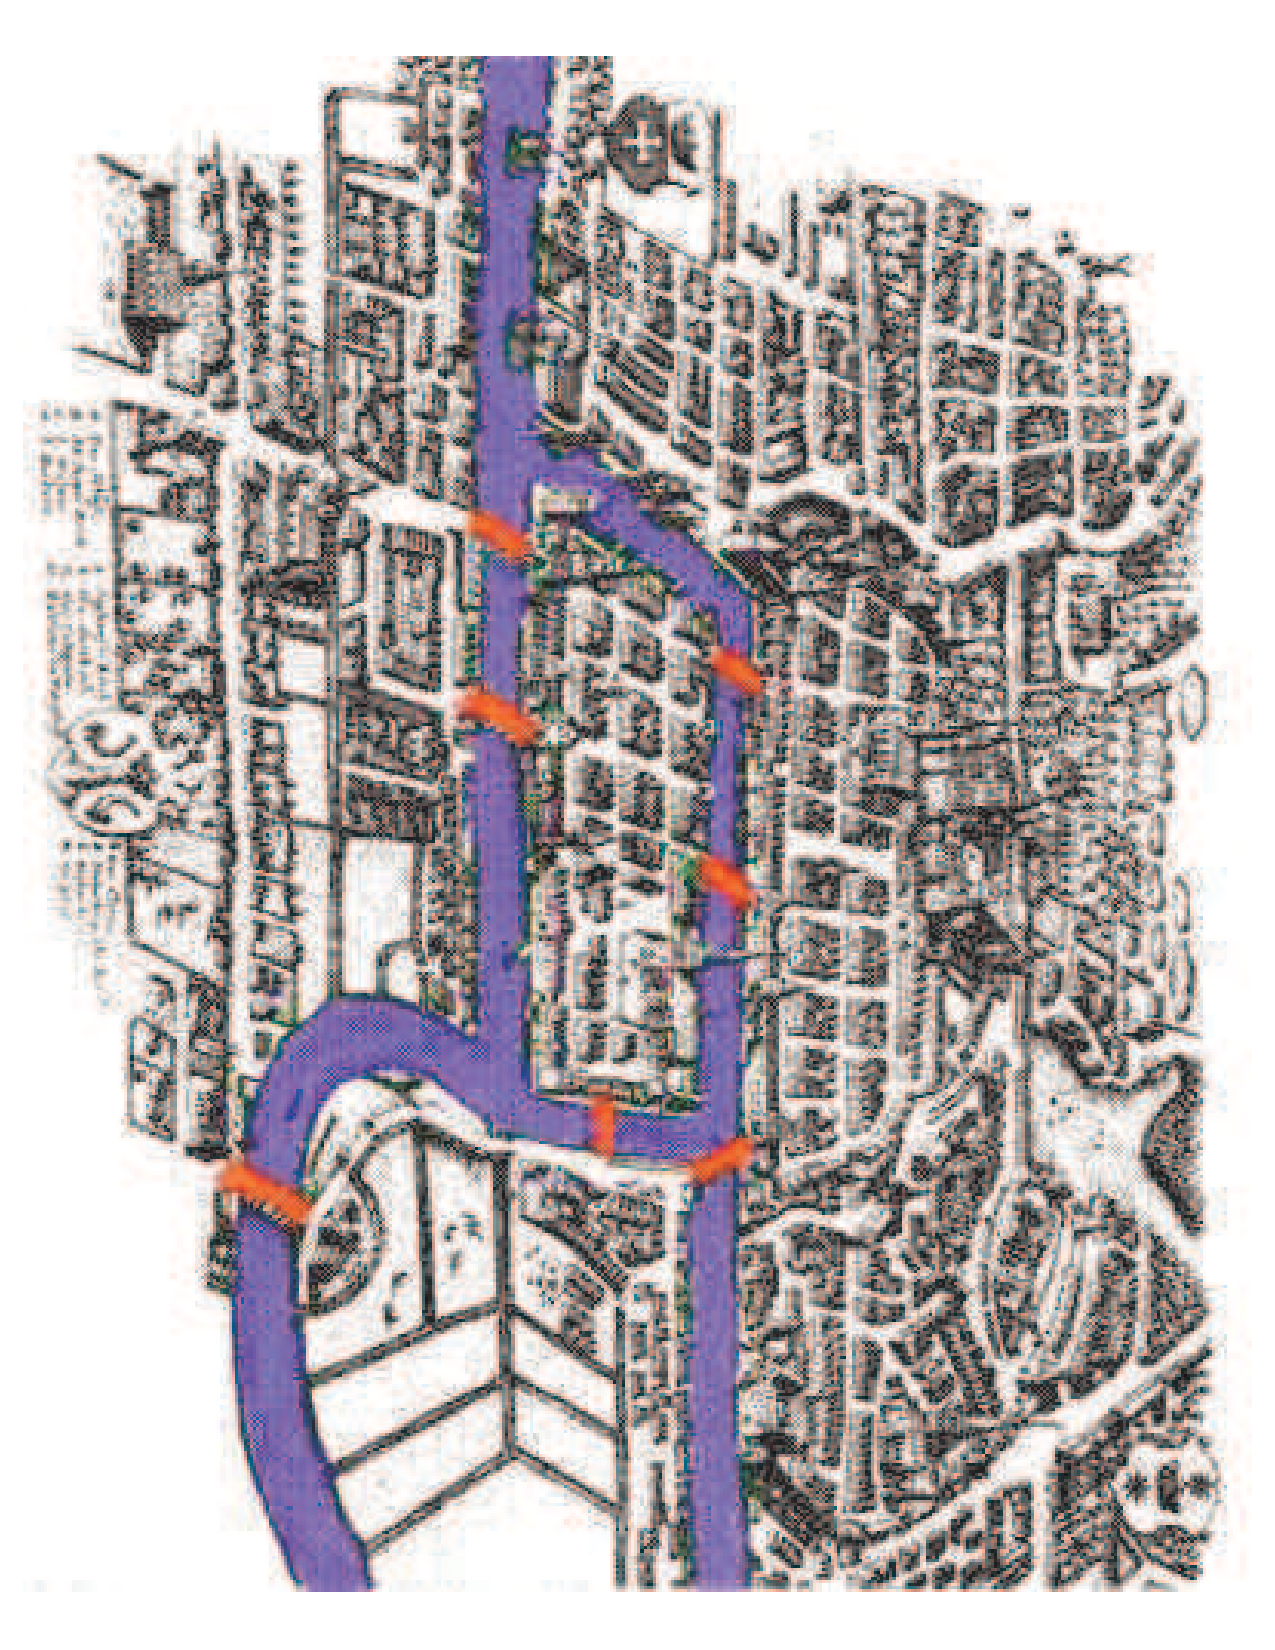
\includegraphics[angle=90,height=.75\textheight]{FIGS/bridge_color}
	\end{center}
\end{frame}

\begin{frame}{The genesis of graphs -- Euler's bridges of K\"onigsberg}
	Cross the 7 bridges in a single walk without recrossing any of them?
	\begin{center}
	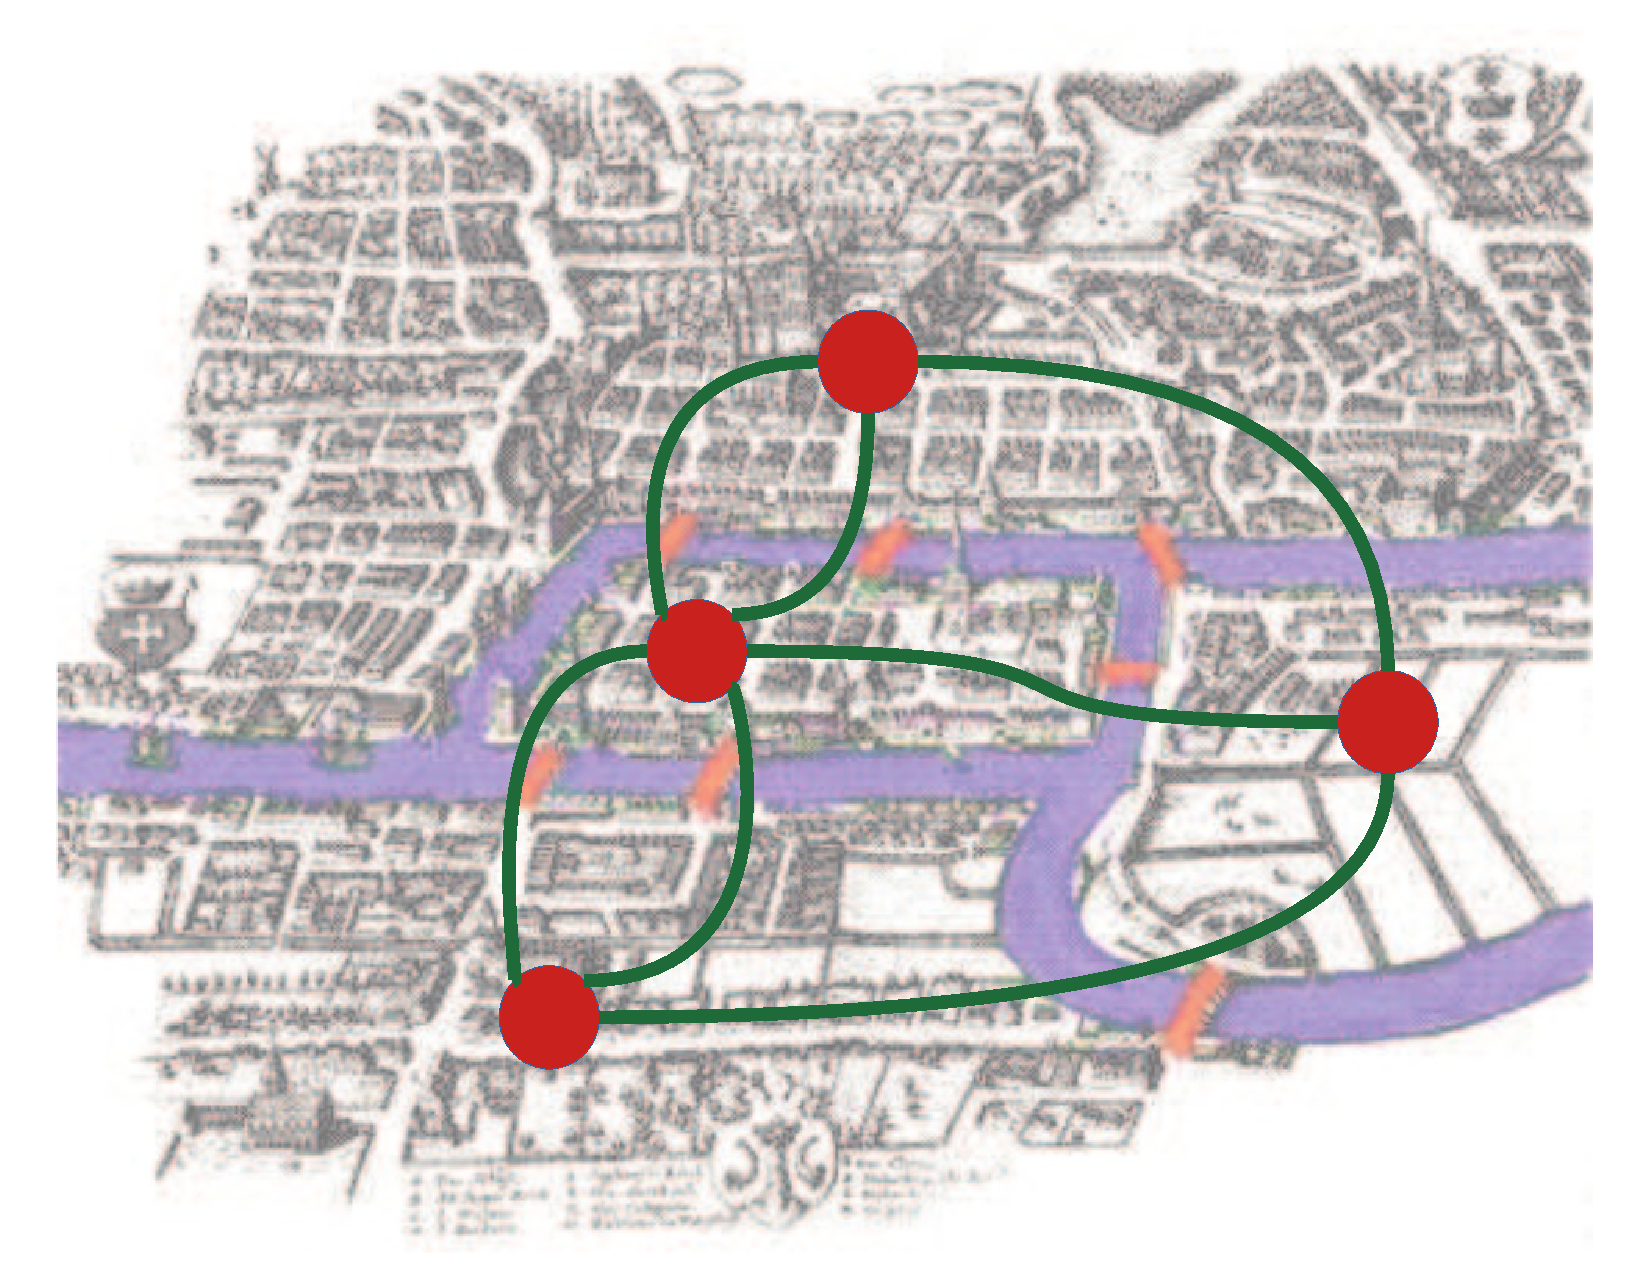
\includegraphics[height=.75\textheight]{FIGS/bridge_color_with_graph}
	\end{center}
\end{frame}

\begin{frame}{The genesis of graphs -- Euler's bridges of K\"onigsberg}
	Cross the 7 bridges in a single walk without recrossing any of them?
	\begin{center}
		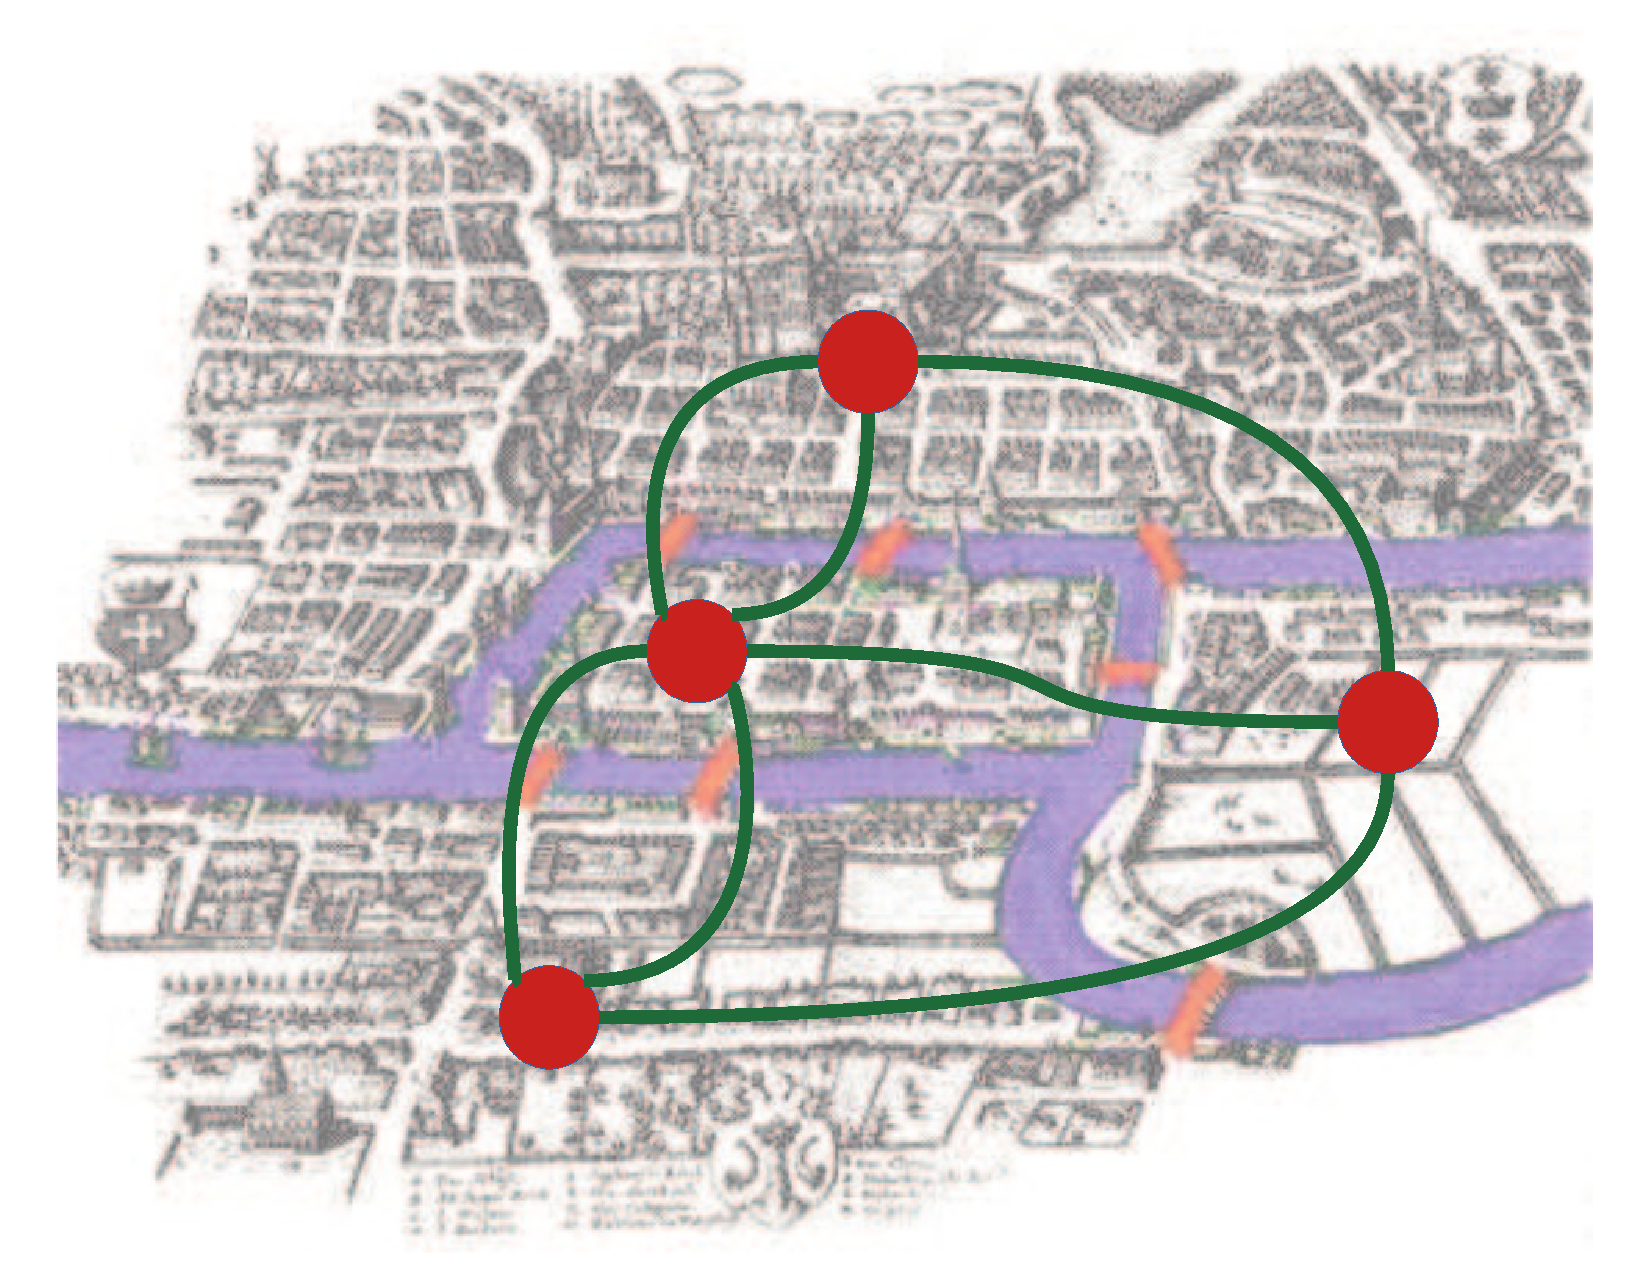
\includegraphics[height=.5\textheight]{FIGS/bridge_color_with_graph}
		\end{center}
	\begin{block}{Mathematical problem}
	Is it possible to find a \emph{trail} containing all \emph{edges} of the graph?
	\end{block}
\end{frame}

\begin{frame}{Finding a cycle with all vertices}
Salesperson must visit some cities (vertices) for their job. Can they plan a round trip using trains enabling them to visit each specified city exactly once?
	\begin{center}
	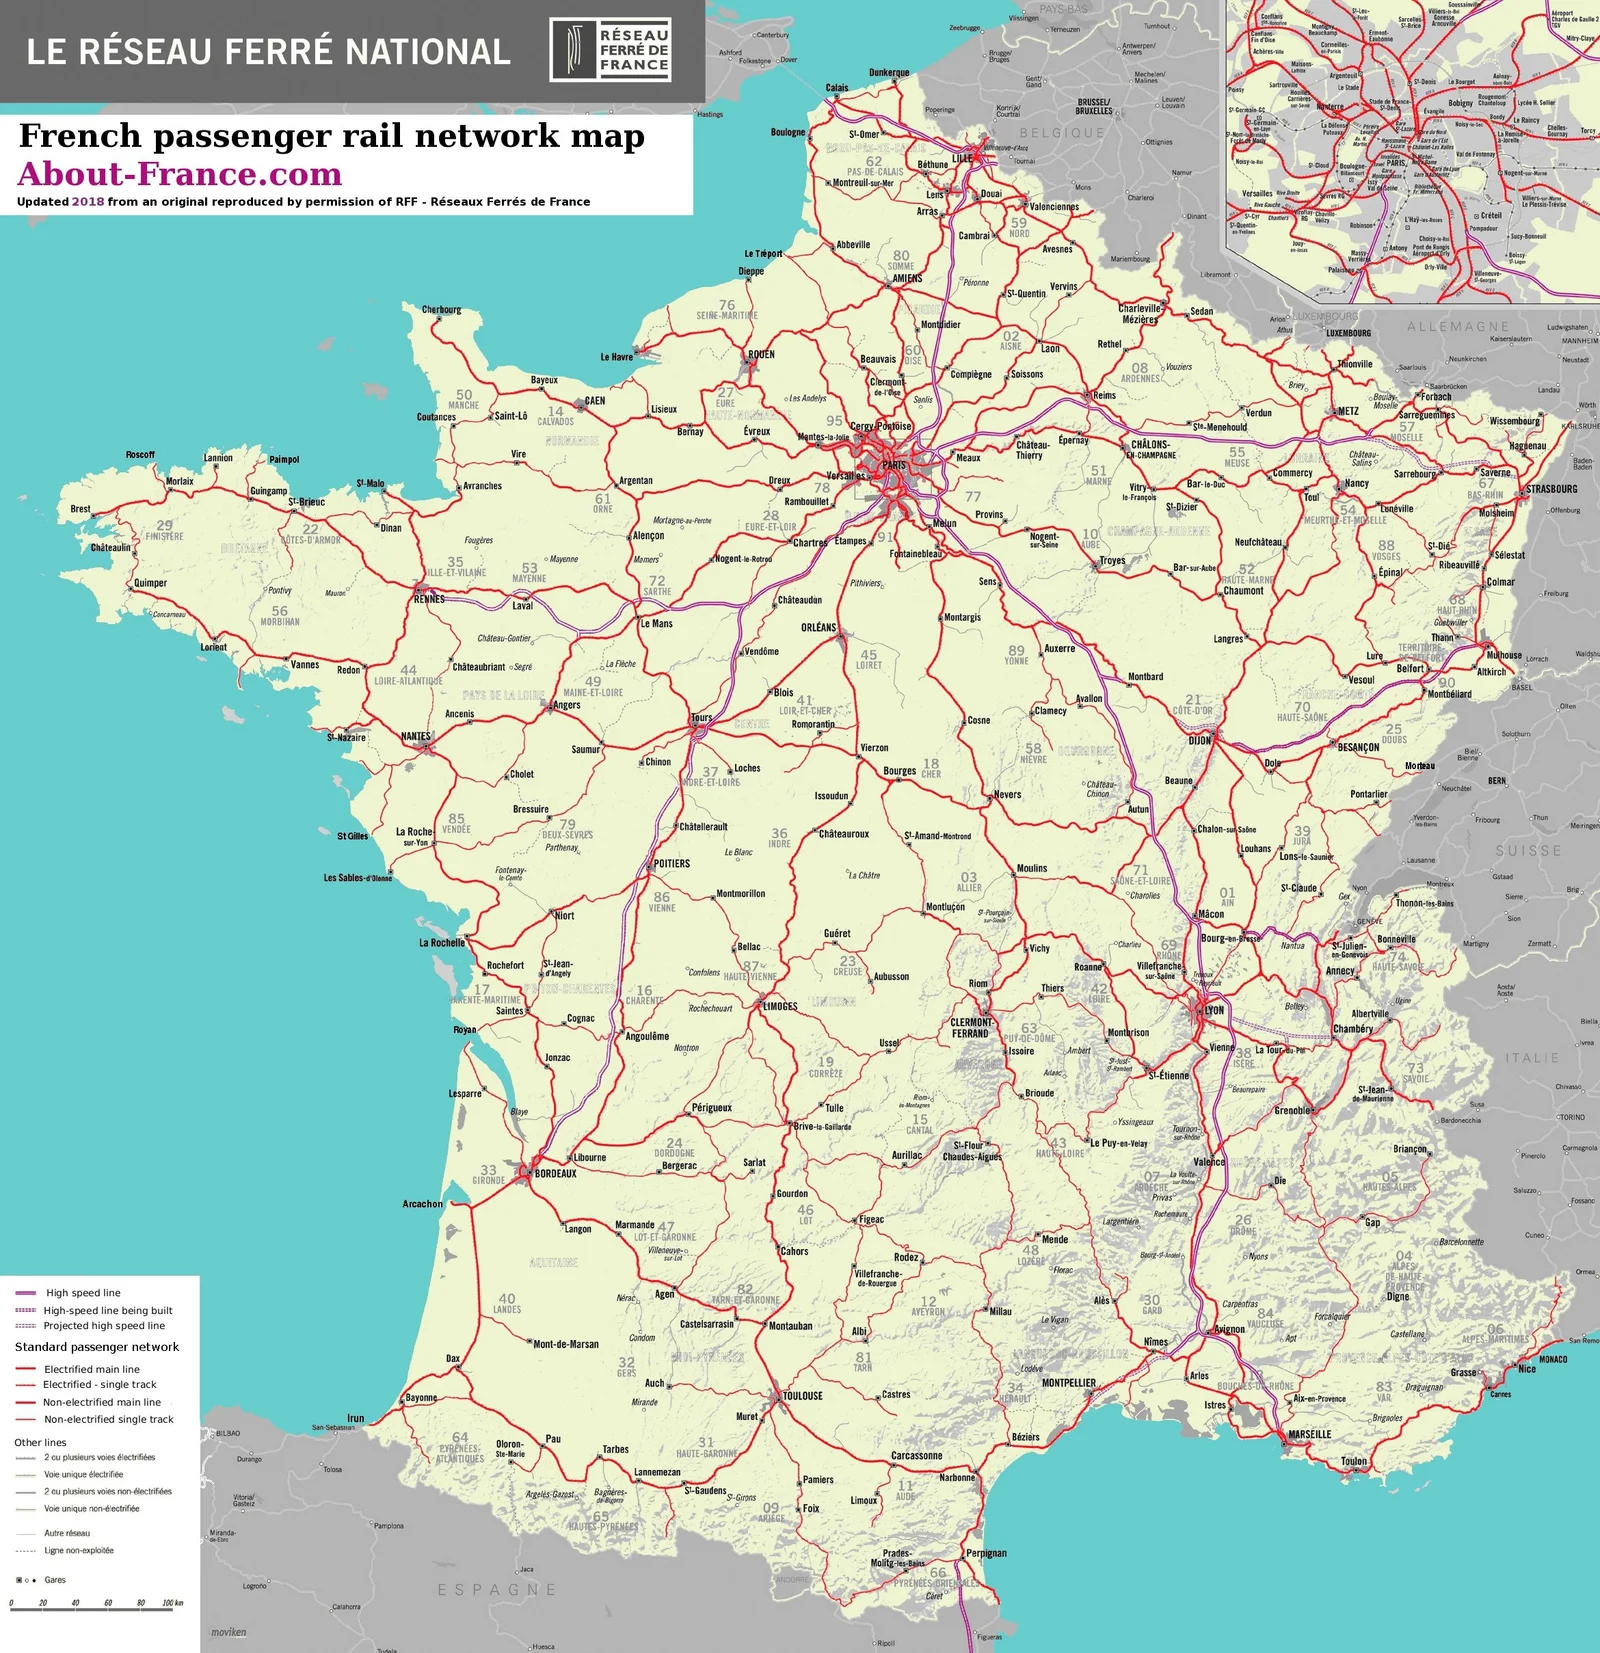
\includegraphics[width=.25\textwidth]{FIGS/RFF-map}
	\end{center}
	\begin{itemize}
	\item 2 vertices are connected iff a line connects the cities and does not pass through any other city
	\end{itemize}
	\begin{block}{Mathematical problem}
	Is it possible to find a cycle containing all graph vertices?
	\end{block}
\end{frame}

\begin{frame}{How far is it to ``train'' through $n$ cities?}
	What is the minimal length of train travel needed to visit $n$ cities (vertices)?
	\begin{center}
	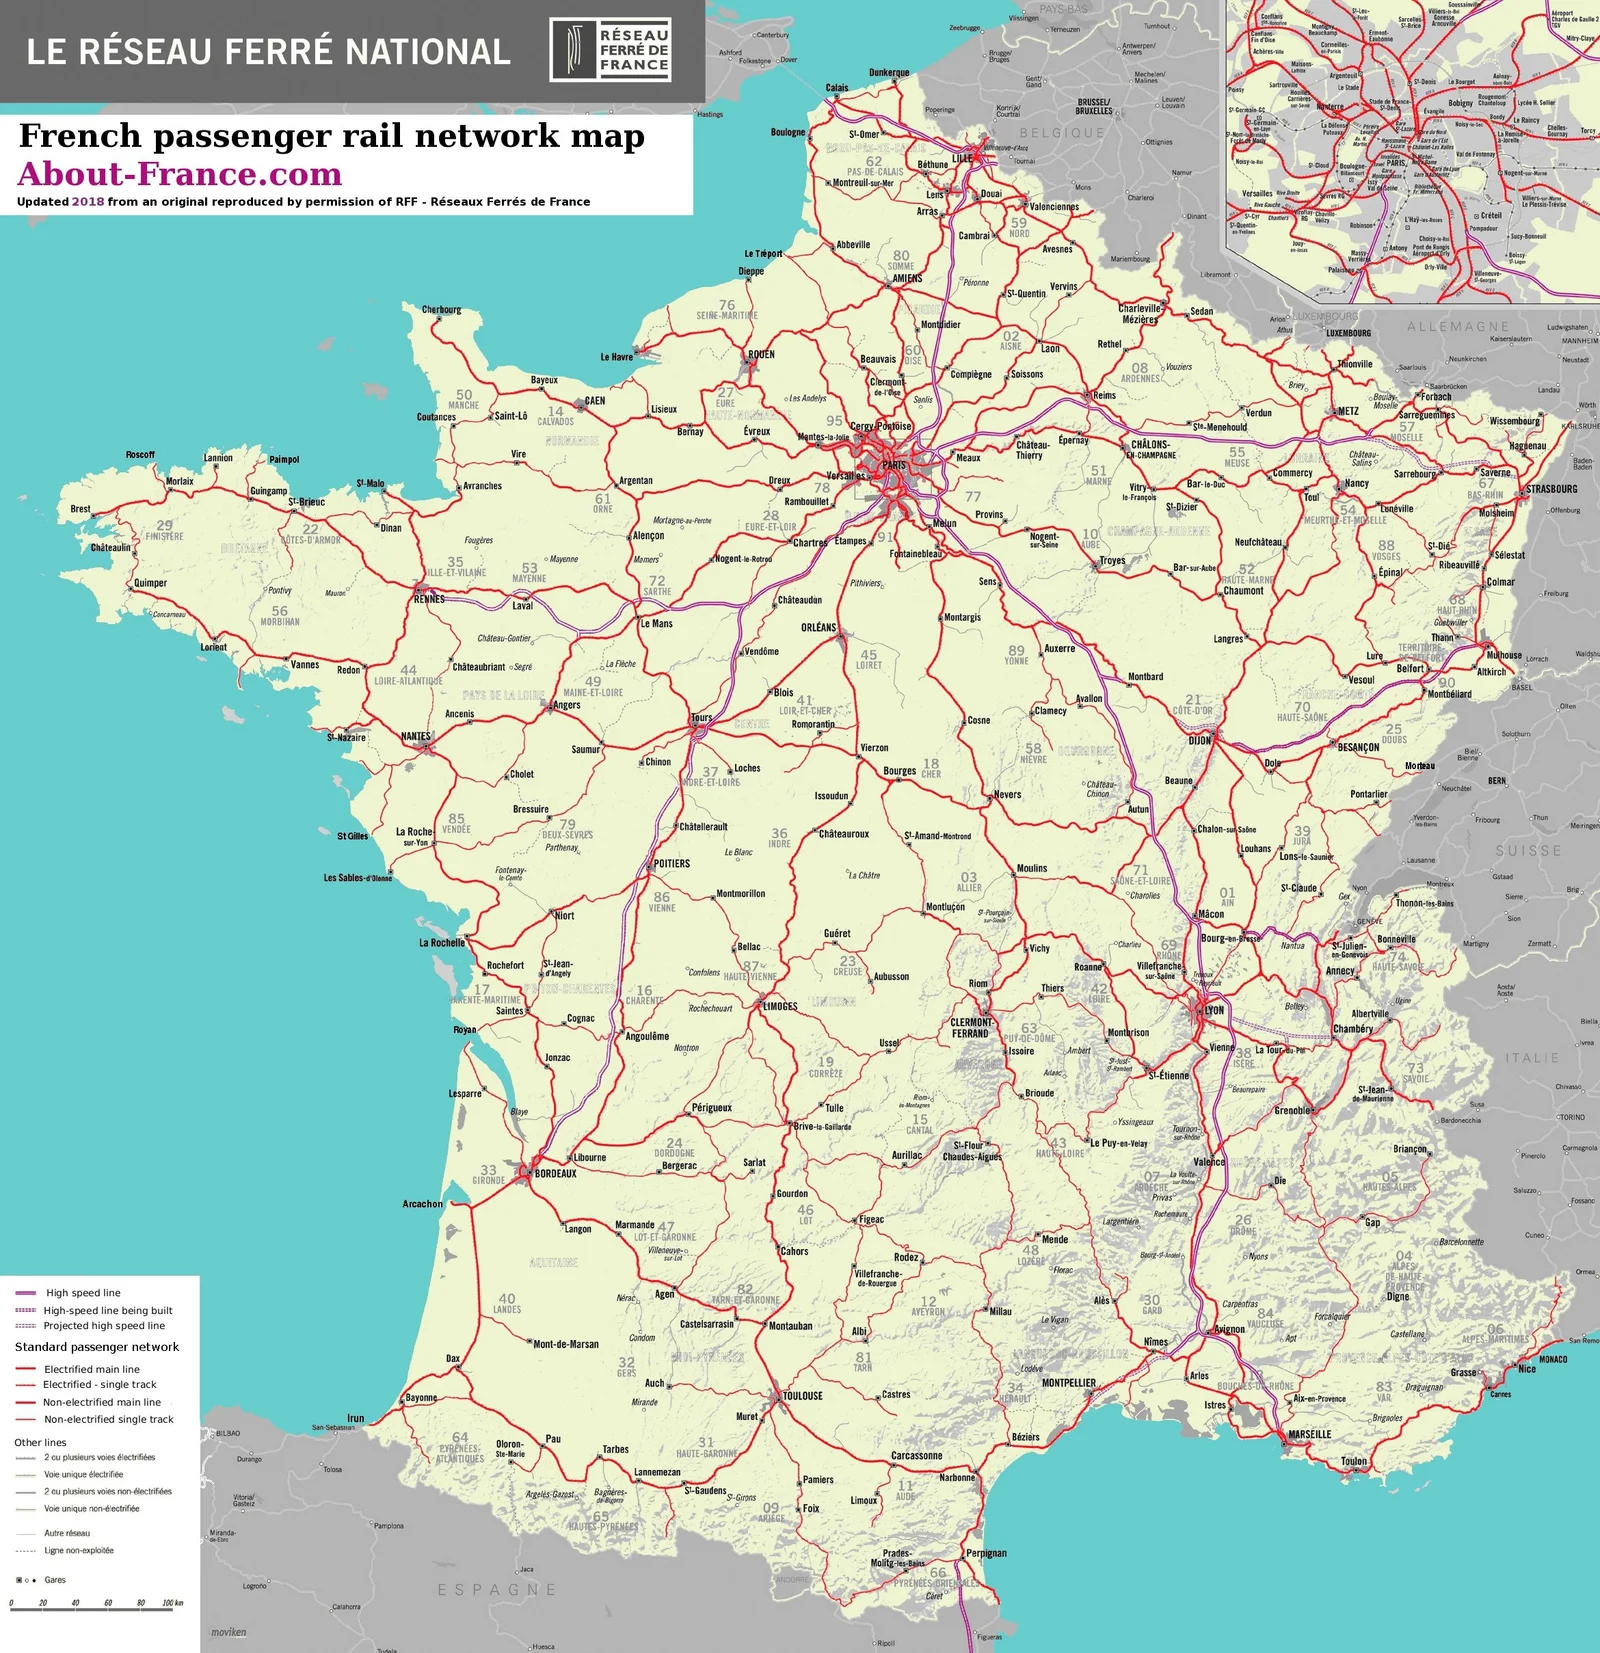
\includegraphics[width=.3\textwidth]{FIGS/RFF-map}
	\end{center}
	\begin{itemize}
	\item all cities are connected; each edge has a value assigned to it (the distance)
	\end{itemize}
	\begin{block}{Mathematical problem}
	What is the minimal spanning tree associated to the graph?
	\end{block}
\end{frame}


\begin{frame}{Graphs/networks encode relations}
	Graphs are used in a variety of contexts because they encode \emph{relations} between objects
	\vfill
	Many objects in the world have relations... so graphs are quite easy to find
	\vfill
	We will see many examples later, for now we cover the mathematical background
\end{frame}



\begin{frame}{Graphs vs digraphs vs multigraphs vs multidigraphs vs ...}
	Name-wise and notation-wise, this domain is a bit of a mess
	\vfill
	\begin{itemize}
		\item The vertex set $V$ is essentially the only constant
		\item \emph{Undirected graph} $G=(V,E)$, where $E$ are the \emph{edges}
		\item \emph{Undirected multigraph} $G_M=(V,E)$
		\item \emph{Directed graph} (or \emph{digraph}) $G=(V,A)$, where $A$ are the \emph{arcs}
		\item \emph{Directed multigraph} (or \emph{multidigraph}) $G_M=(V,A)$
		\item Any of the above is called a \emph{graph} and is denoted $G=(V,X)$, when we seek generality
	\end{itemize}
	\vfill
And just to confuse the whole thing more: we often say \emph{graph} for \emph{unoriented graph}
\end{frame}

%%%%%%%%%%%%%%%%%%%%
%%%%%%%%%%%%%%%%%%%%
%%%%%%%%%%%%%%%%%%%%
%%%%%%%%%%%%%%%%%%%%
\section{Binary relations}
\newSectionSlide{FIGS-slides-admin/Gemini_Generated_Image_fto8nofto8nofto8.jpeg}


\begin{frame}\frametitle{Binary relation}
	\begin{definition}[Binary relation]
	\begin{itemize}
	\item A \defword{binary relation} is an arbitrary association of elements of one set with elements of another (maybe the same) set
	\item  A binary relation over the sets $X$ and $Y$ is defined as a subset of the Cartesian product $X\times Y =\{(x,y)| x\in X , y\in Y\}$
	\item $(x,y)\in R$ is read ``$x$ is $R$-related to $y$'' and is denoted $xRy$
	\item If $(x,y)\not\in R$, we write ``not $x R y$'' or $x\cancel{R} y$
	\end{itemize}
	\end{definition}
\end{frame}
	
\begin{frame}
	\begin{definition}[Properties of binary relations]
		A binary relation $R$ over a set $X$ is
	\begin{itemize}
	\item \defword{Reflexive} if $\forall x\in X$, $xRx$
	\item \defword{Irreflexive} if there does not exist $x\in X$ such that $xRx$
	\item \defword{Symmetric} if $xRy \Rightarrow yRx$
	\item \defword{Asymmetric} if $xRy \Rightarrow $ $y\cancel R x$
	\item \defword{Antisymmetric} if $xRy$ and $yRx$ $\Rightarrow$ $x=y$
	\item \defword{Transitive} if $xRy$ and $yRz$ $\Rightarrow$  $xRz$
	\item \defword{Total} (or \defword{complete}) if $\forall x, y\in X$, $x R y$ or $y R x$
	\end{itemize}
	\end{definition}
\end{frame}
	
	
\begin{frame} 
	\begin{definition}[Equivalence relation]
	 A relation that is reflexive ($\forall x\in X$, $xRx$), symmetric ($xRy \Rightarrow yRx$) and transitive ($xRy$ and $yRz$ $\Rightarrow$  $xRz$) is an \defword{equivalence relation}
	\end{definition}
	\vfill
	\begin{definition}[Partial order]
	 A relation that is reflexive ($\forall x\in X$, $xRx$), antisymmetric ($xRy$ and $yRx$ $\Rightarrow$ $x=y$) and transitive ($xRy$ and $yRz$ $\Rightarrow$  $xRz$) is a \defword{partial order}
	\end{definition}
	\vfill
	\begin{definition}[Total order]
	A partial order that is total ($\forall x, y\in X$, $x R y$ or $y R x$) is a \defword{total order}
	\end{definition}
\end{frame}
	



%%%%%%%%%%%%%%%%%%%%
%%%%%%%%%%%%%%%%%%%%
%%%%%%%%%%%%%%%%%%%%
%%%%%%%%%%%%%%%%%%%%
\section{Undirected graphs}
\newSectionSlide{FIGS-slides-admin/Gemini_Generated_Image_fto8nofto8nofto8.jpeg}


\begin{frame}\frametitle{The \code{igraph} library}
Throughout these slides, we use the package \code{igraph}
\vfill
I illustrate the functions that can be used to study some of the mathematical notions I introduce
\vfill
I use mostly examples from the \code{igraph} documentation
\end{frame}


\subsection{Undirected graph}
\newSubSectionSlide{FIGS-slides-admin/Gemini_Generated_Image_fto8nofto8nofto8.jpeg}


\begin{frame}{Graph}
	Intuitively: a graph is a set of points, and a set of relations between the points
	\vfill
	The points are called the \emph{vertices} of the graph and the relations are the \emph{edges} of the graph
	\vfill
	We can also think of the relations as being one directional, in which case the relations are the \emph{arcs} of the digraph (a contraction of ``directed graph'')
\end{frame}


\begin{frame}\frametitle{Graph, vertex and edge} 
	\begin{definition}[Graph]
	An \defword{undirected graph} is a pair $G=(V,E)$ of sets such that
	\begin{itemize}
	\item $V$ is a set of points:  $V=\{v_1,\ldots,v_p\}$
	\item $E$ is a set of 2-element subsets of $V$: $E=\{\{v_i,v_j\},\{v_i,v_k\},\ldots,\{v_n,v_p\}\}$ or $E=\{v_iv_j,v_iv_k,\ldots,v_nv_p\}$
	\end{itemize}
	\end{definition}
	\begin{definition}[Vertex]
	The elements of $V$ are the \defword{vertices} (or nodes, or points) of the graph $G$.
	$V$ (or $V(G)$) is the vertex set of the graph $G$
	\end{definition}
	\begin{definition}[Edge]
	The elements of $E$ are the \defword{edges} (or lines) of the graph $G$.
	$E$ (or $E(G)$) is the edge set of the graph $G$
	\end{definition}
\end{frame}


\begin{frame}[fragile]\frametitle{Setting up graphs in \code{igraph}}
\begin{knitrout}
\definecolor{shadecolor}{rgb}{0.969, 0.969, 0.969}\color{fgcolor}\begin{kframe}
\begin{alltt}
\hldef{G} \hlkwb{<-} \hlkwd{make_empty_graph}\hldef{()}
\hldef{G} \hlkwb{<-} \hlkwd{make_graph}\hldef{(}\hlkwc{edges} \hldef{=} \hlkwd{c}\hldef{(}\hlnum{1}\hldef{,} \hlnum{2}\hldef{,} \hlnum{1}\hldef{,} \hlnum{5}\hldef{),} \hlkwc{n} \hldef{=} \hlnum{10}\hldef{,}
                \hlkwc{directed} \hldef{=} \hlnum{FALSE}\hldef{)}
\hldef{G} \hlkwb{<-} \hlkwd{make_graph}\hldef{(}\hlsng{"Zachary"}\hldef{)}
\hlkwd{plot}\hldef{(G,} \hlkwc{main} \hldef{=} \hlsng{"Data on a Karate club"}\hldef{)}
\end{alltt}
\end{kframe}
\end{knitrout}
\end{frame}

\maxFrameImage{FIGS/L15-setup-graph-1-1.pdf}

\begin{frame}\frametitle{Order and Size}
	\begin{definition}[Order of a graph]
	The number of vertices in $G$ is the \defword{order} of $G$. Using the notation $|V(G)|$ for the \emph{cardinality} of $V(G)$,
	$$|V(G)|=\textrm{order of G}$$
	\end{definition}
	\vfill
	\begin{definition}[Size of a graph]
	The number of edges in $G$ is the \defword{size} of $G$,
	$$|E(G)|=\textrm{size of G}$$
	\end{definition}
	\vfill
	\begin{itemize}
	\item A graph having order $p$ and size $q$ is called a $(p,q)-$graph
	\item A graph is finite if $|V(G)|<\infty$
	\end{itemize}
\end{frame}

\begin{frame}[fragile]\frametitle{Some simple measures}
\begin{knitrout}
\definecolor{shadecolor}{rgb}{0.969, 0.969, 0.969}\color{fgcolor}\begin{kframe}
\begin{alltt}
\hlkwd{V}\hldef{(G)}
\end{alltt}
\begin{verbatim}
## + 34/34 vertices, from b79af2b:
##  [1]  1  2  3  4  5  6  7  8  9 10 11 12 13 14 15 16 17 18 19 20 21 22 23 24 25
## [26] 26 27 28 29 30 31 32 33 34
\end{verbatim}
\begin{alltt}
\hlkwd{head}\hldef{(}\hlkwd{E}\hldef{(G))}
\end{alltt}
\begin{verbatim}
## + 6/78 edges from b79af2b:
## [1] 1--2 1--3 1--4 1--5 1--6 1--7
\end{verbatim}
\begin{alltt}
\hlkwd{gorder}\hldef{(G)}
\end{alltt}
\begin{verbatim}
## [1] 34
\end{verbatim}
\begin{alltt}
\hlkwd{gsize}\hldef{(G)}
\end{alltt}
\begin{verbatim}
## [1] 78
\end{verbatim}
\end{kframe}
\end{knitrout}
\end{frame}

\begin{frame}\frametitle{Incident -- Adjacent}
	\begin{definition}[Incident]
	\begin{itemize}
	\item A vertex $v$ is \defword{incident} with an edge $e$ if $v\in e$; then $e$ is an edge at $v$
	\item If $e=uv\in E(G)$, then $u$ and $v$ are each incident with $e$
	\item The two vertices incident with an edge are its ends
	\item An edge $e=uv$ is incident with both vertices $u$ and $v$
	\end{itemize}
	\end{definition}
	\vfill
	\begin{definition}[Adjacent]
	\begin{itemize}
	\item Two vertices $u$ and $v$ are \defword{adjacent} in a graph $G$ if $uv\in E(G)$
	\item If $uv$ and $uw$ are distinct edges (i.e. $v\not=w$) of a graph $G$, then $uv$ and $uw$ are adjacent edges
	\end{itemize}
	\end{definition}
\end{frame}


\begin{frame}[fragile]\frametitle{Incident vertices}
\begin{knitrout}
\definecolor{shadecolor}{rgb}{0.969, 0.969, 0.969}\color{fgcolor}\begin{kframe}
\begin{alltt}
\hlkwd{incident}\hldef{(G,} \hlnum{1}\hldef{)}
\end{alltt}
\begin{verbatim}
## + 16/78 edges from b79af2b:
##  [1] 1-- 2 1-- 3 1-- 4 1-- 5 1-- 6 1-- 7 1-- 8 1-- 9 1--11 1--12 1--13 1--14
## [13] 1--18 1--20 1--22 1--32
\end{verbatim}
\begin{alltt}
\hlkwd{incident_edges}\hldef{(G,} \hlkwd{c}\hldef{(}\hlnum{1}\hldef{,} \hlnum{2}\hldef{))}
\end{alltt}
\begin{verbatim}
## [[1]]
## + 16/78 edges from b79af2b:
##  [1] 1-- 2 1-- 3 1-- 4 1-- 5 1-- 6 1-- 7 1-- 8 1-- 9 1--11 1--12 1--13 1--14
## [13] 1--18 1--20 1--22 1--32
## 
## [[2]]
## + 9/78 edges from b79af2b:
## [1] 1-- 2 2-- 3 2-- 4 2-- 8 2--14 2--18 2--20 2--22 2--31
\end{verbatim}
\end{kframe}
\end{knitrout}
\end{frame}

\begin{frame}[fragile]\frametitle{Adjacent vertices}
\begin{knitrout}
\definecolor{shadecolor}{rgb}{0.969, 0.969, 0.969}\color{fgcolor}\begin{kframe}
\begin{alltt}
\hlkwd{adjacent_vertices}\hldef{(G,} \hlkwc{v} \hldef{=} \hlnum{1}\hldef{)}
\end{alltt}
\begin{verbatim}
## [[1]]
## + 16/34 vertices, from b79af2b:
##  [1]  2  3  4  5  6  7  8  9 11 12 13 14 18 20 22 32
\end{verbatim}
\begin{alltt}
\hlkwd{adjacent_vertices}\hldef{(G,} \hlkwc{v} \hldef{=} \hlkwd{c}\hldef{(}\hlnum{1}\hldef{,} \hlnum{2}\hldef{))}
\end{alltt}
\begin{verbatim}
## [[1]]
## + 16/34 vertices, from b79af2b:
##  [1]  2  3  4  5  6  7  8  9 11 12 13 14 18 20 22 32
## 
## [[2]]
## + 9/34 vertices, from b79af2b:
## [1]  1  3  4  8 14 18 20 22 31
\end{verbatim}
\end{kframe}
\end{knitrout}
\end{frame}


\begin{frame}
	\begin{definition}[Multiple edge]
	\defword{Multiple edges} are two or more edges connecting the same two vertices within a multigraph
	\end{definition}
	\vfill
	\begin{definition}[Loop]
	A \defword{loop} is an edge with both the same ends; \emph{e.g.} $\{u,u\}$ is a loop
	\end{definition}
	\vfill
	\begin{definition}[Simple graph]
		A \defword{simple graph} is a graph which contains no loops or multiple edges
	\end{definition}
	\vfill
	\begin{definition}[Multigraph]
		A \defword{multigraph} is a graph which can contain multiple edges or loops
	\end{definition}
\end{frame}


\begin{frame}[fragile]\frametitle{Testing for these properties}
\begin{knitrout}
\definecolor{shadecolor}{rgb}{0.969, 0.969, 0.969}\color{fgcolor}\begin{kframe}
\begin{alltt}
\hlkwd{any_multiple}\hldef{(G)}
\end{alltt}
\begin{verbatim}
## [1] FALSE
\end{verbatim}
\begin{alltt}
\hlkwd{any_loop}\hldef{(G)}
\end{alltt}
\begin{verbatim}
## [1] FALSE
\end{verbatim}
\begin{alltt}
\hlkwd{is_simple}\hldef{(G)}
\end{alltt}
\begin{verbatim}
## [1] TRUE
\end{verbatim}
\end{kframe}
\end{knitrout}
\end{frame}



\begin{frame}\frametitle{Graph and binary relations}
A simple graph $G$ can be defined in term of a vertex set $V$ and a binary relation over $V$ that is
	\begin{itemize}
		\item irreflexive ($\forall u\in V$, $u\cancel Ru$)
		\item symmetric ($\forall u,v\in V$, $uRv\implies vRu$)
	\end{itemize}
	\vfill
	The set of edges $E(G)$ is the set of symmetric pairs in $R$
	\vfill
	If $R$ is not irreflexive, the graph is not simple
\end{frame}


\subsection{Degree of a vertex}
\newSubSectionSlide{FIGS-slides-admin/Gemini_Generated_Image_fto8nofto8nofto8.jpeg}

\begin{frame}
	\begin{definition}[Degree of a vertex]
	Let $v$ be a vertex of $G=(V,E)$.
	\begin{itemize}
	\item The number of edges of $G$ incident with $v$ is the \defword{degree} of $v$ in $G$
	\item The number of edges of $G$ at $v$ is the \defword{degree} of $v$ in $G$
	\item The degree of $v$ in $G$ is noted $d_G(v)$ or $deg_G(v)$
	\end{itemize}
	\end{definition}
	\vfill
	\begin{theorem}\label{th:sum-degrees}
	Let $G$ be a $(p,q)-$graph with vertices $v_1$, $\dots$, $v_p$, then
	\[
		\sum_{i=1}^{p}d_G(v_i)=2q
	\]
	\end{theorem}
\end{frame}

\begin{frame}[fragile]\frametitle{Degree}
\begin{knitrout}
\definecolor{shadecolor}{rgb}{0.969, 0.969, 0.969}\color{fgcolor}\begin{kframe}
\begin{alltt}
\hlkwd{degree}\hldef{(G)}
\end{alltt}
\begin{verbatim}
##  [1] 16  9 10  6  3  4  4  4  5  2  3  1  2  5  2  2  2  2  2  3  2  2  2  5  3
## [26]  3  2  4  3  4  4  6 12 17
\end{verbatim}
\begin{alltt}
\hlkwd{degree_distribution}\hldef{(G)}
\end{alltt}
\begin{verbatim}
##  [1] 0.00000000 0.02941176 0.32352941 0.17647059 0.17647059 0.08823529
##  [7] 0.05882353 0.00000000 0.00000000 0.02941176 0.02941176 0.00000000
## [13] 0.02941176 0.00000000 0.00000000 0.00000000 0.02941176 0.02941176
\end{verbatim}
\begin{alltt}
\hlkwd{plot}\hldef{(}\hlkwd{degree_distribution}\hldef{(G),}
     \hlkwc{type} \hldef{=} \hlsng{"b"}\hldef{,}
     \hlkwc{xlab} \hldef{=} \hlsng{"Degree"}\hldef{,} \hlkwc{ylab} \hldef{=} \hlsng{"Frequency"}\hldef{,}
     \hlkwc{main} \hldef{=} \hlsng{"Degree distribution of the Karate graph"}\hldef{)}
\end{alltt}
\end{kframe}
\end{knitrout}
\end{frame}

\maxFrameImage{FIGS/L15-vertex-degrees-undirected-1.pdf}



\begin{frame}
\begin{definition}[{Odd vertex}]
A vertex is an \defword{odd vertex} is its degree is odd
\end{definition}
\vfill
\begin{definition}[{Even vertex}]
A vertex is called \defword{even vertex} is its degree is even
\end{definition}
\vfill
\begin{theorem}\label{th:even-nb-odd-vertices}
Every graph contains an even number of odd vertices
\end{theorem}
\end{frame}

\begin{frame}[fragile]\frametitle{Illustration of recent results}
Theorem~\ref{th:sum-degrees} states that a $(p,q)-$graph has $\sum_{i=1}^{p}d_G(v_i)=2q$
\begin{knitrout}
\definecolor{shadecolor}{rgb}{0.969, 0.969, 0.969}\color{fgcolor}\begin{kframe}
\begin{alltt}
\hlkwd{sum}\hldef{(}\hlkwd{degree}\hldef{(G))} \hlopt{==} \hlnum{2}\hlopt{*}\hlkwd{length}\hldef{(}\hlkwd{E}\hldef{(G))}
\end{alltt}
\begin{verbatim}
## [1] TRUE
\end{verbatim}
\end{kframe}
\end{knitrout}
\vfill
Theorem~\ref{th:even-nb-odd-vertices} states that every graph contains an even number of odd vertices
\begin{knitrout}
\definecolor{shadecolor}{rgb}{0.969, 0.969, 0.969}\color{fgcolor}\begin{kframe}
\begin{alltt}
\hlkwd{sum}\hldef{(pracma}\hlopt{::}\hlkwd{mod}\hldef{(}\hlkwd{degree}\hldef{(G),}\hlnum{2}\hldef{))}
\end{alltt}
\begin{verbatim}
## [1] 12
\end{verbatim}
\end{kframe}
\end{knitrout}
(\code{mode(x,2)} returns 1 if $x$ is odd so \code{sum} counts how many are odd)
\end{frame}

\begin{frame}[fragile]{Regular graph}
\begin{definition}[{Regular graph}]
	If all the vertices of $G$ have the same degree $k$, then the graph $G$ is $k$-regular
\end{definition}
\vfill
\begin{knitrout}
\definecolor{shadecolor}{rgb}{0.969, 0.969, 0.969}\color{fgcolor}\begin{kframe}
\begin{alltt}
\hlkwd{length}\hldef{(}\hlkwd{unique}\hldef{(}\hlkwd{degree}\hldef{(G)))} \hlopt{==} \hlnum{1}
\end{alltt}
\begin{verbatim}
## [1] FALSE
\end{verbatim}
\end{kframe}
\end{knitrout}
\end{frame}




%%%%%%%%%%%%%%%%%%%%%%%
%%%%%%%%%%%%%%%%%%%%%%%
\subsection{Isomorphic graphs}
\newSubSectionSlide{FIGS-slides-admin/Gemini_Generated_Image_fto8nofto8nofto8.jpeg}

\begin{frame} \frametitle{Isomorphic graphs} 
\begin{definition}[Isomorphic graphs]
Let $G_1=(V(G_1),E(G_1))$ and $G_2=(V(G_2),E(G_2))$ be two graphs.
$G_1$ and $G_2$ are \defword{isomorphic} if there exists an isomorphism $\phi$ from $G_1$ to $G_2$, that is defined as an injective mapping $\phi:\; V(G_1) \rightarrow V(G_2)$ such that two vertices $u_1$ and $v_1$ are adjacent in $G_1$ $\iff$ the vertices $\phi(u_1)$ and $\phi(v_1)$ are adjacent in $G_2$
\end{definition}
\end{frame}
 
 
 
\begin{frame}
If $\phi$ is an isomorphism from $G_1$ to $G_2$, then the inverse mapping $\phi ^{-1}$ from $V(G_2)$ to $V(G_1)$ also satisfies the definition of an isomorphism.
As a consequence, if $G_1$ and $G_2$ are isomorphic graphs, then
\begin{itemize}
\item $G_1$ is isomorphic to $G_2$
\item $G_2$ is isomorphic to $G_1$
\end{itemize}
\vfill
\begin{theorem}
The relation ``is isomorphic to'' is an equivalence relation on the set of all graphs
\end{theorem}
\vfill
\begin{theorem}
If $G_1$ and $G_2$ are isomorphic graphs, then the degrees of vertices of $G_1$ are exactly the degrees of vertices of $G_2$
\end{theorem}
\end{frame}

\begin{frame}[fragile]\frametitle{Testing isomorphicity}
Create two isomorphic graphs by permuting the vertices of the first, then test if they are isomorphic
\vfill
\begin{knitrout}
\definecolor{shadecolor}{rgb}{0.969, 0.969, 0.969}\color{fgcolor}\begin{kframe}
\begin{alltt}
\hldef{g1} \hlkwb{<-} \hlkwd{sample_pa}\hldef{(}\hlnum{30}\hldef{,} \hlkwc{m} \hldef{=} \hlnum{2}\hldef{,} \hlkwc{directed} \hldef{=} \hlnum{FALSE}\hldef{)}
\hldef{g2} \hlkwb{<-} \hlkwd{permute}\hldef{(g1,} \hlkwd{sample}\hldef{(}\hlkwd{vcount}\hldef{(g1)))}
\hlcom{# should be TRUE}
\hlkwd{isomorphic}\hldef{(g1, g2)}
\end{alltt}
\begin{verbatim}
## [1] TRUE
\end{verbatim}
\end{kframe}
\end{knitrout}
\end{frame}


%%%%%%%%%%%%%%%%%%%%%%%
%%%%%%%%%%%%%%%%%%%%%%%
\subsection{Subgraphs, unions of graphs}
\newSubSectionSlide{FIGS-slides-admin/Gemini_Generated_Image_fto8nofto8nofto8.jpeg}

\begin{frame}\frametitle{Subgraph}
\begin{definition}[Subgraph]
Let $G=(V,E)$ be a graph.
A graph $H=(V(H),E(H))$ is a \defword{subgraph} of $G$ if $V(H)\subseteq V$ and $E(H)\subseteq E$
\end{definition}
\end{frame}

\begin{frame}[fragile]\frametitle{Extracting a subgraph}
\begin{knitrout}
\definecolor{shadecolor}{rgb}{0.969, 0.969, 0.969}\color{fgcolor}\begin{kframe}
\begin{alltt}
\hldef{G_sub} \hlkwb{=} \hlkwd{induced_subgraph}\hldef{(G,} \hlkwd{c}\hldef{(}\hlnum{1}\hlopt{:}\hlnum{5}\hldef{,} \hlnum{11}\hlopt{:}\hlnum{14}\hldef{))}
\hlkwd{plot}\hldef{(G_sub,} \hlkwc{main} \hldef{=} \hlsng{"A subgraph of the Karate graph"}\hldef{)}
\end{alltt}
\end{kframe}
\end{knitrout}
\end{frame}

\maxFrameImage{FIGS/L15-extract-subgraph-1.pdf}

\begin{frame}[fragile]\frametitle{Naming vertices}
Note that vertices (and as a consequence, edges) will be relabelled, so \code{G\_sub} has vertices labelled 1 to 9
\vfill
You can name vertices if you want to avoid this
\begin{knitrout}
\definecolor{shadecolor}{rgb}{0.969, 0.969, 0.969}\color{fgcolor}\begin{kframe}
\begin{alltt}
\hlkwd{V}\hldef{(G)}\hlopt{$}\hldef{name} \hlkwb{=} \hlnum{1}\hlopt{:}\hlkwd{length}\hldef{(}\hlkwd{V}\hldef{(G))}
\hldef{G_sub} \hlkwb{=} \hlkwd{induced_subgraph}\hldef{(G,} \hlkwd{c}\hldef{(}\hlnum{1}\hlopt{:}\hlnum{5}\hldef{,} \hlnum{11}\hlopt{:}\hlnum{14}\hldef{))}
\hlkwd{plot}\hldef{(G_sub,} \hlkwc{labels} \hldef{=} \hlkwd{V}\hldef{(G)}\hlopt{$}\hldef{name,}
     \hlkwc{main} \hldef{=} \hlsng{"Subgraph of the Karate graph preserving names"}\hldef{)}
\end{alltt}
\end{kframe}
\end{knitrout}
\end{frame}

\maxFrameImage{FIGS/L15-subgraph-named-vertices-1.pdf}


\begin{frame}
Let $G_1=(V_1,E_1)$ and $G_2=(V_2,E_2)$ be two graphs
\begin{definition}[{Union of $G_1$ and $G_2$}]
$G_1\cup G_2=(V_1\cup V_2,E_1\cup E_2)$
\end{definition}
\begin{definition}[{Intersection of $G_1$ and $G_2$}]
$G_1\cap G_2=(V_1\cap V_2,E_1\cap E_2)$
\end{definition}
\begin{definition}[{Disjoint graphs}]
If $G_1\cap G_2=(\emptyset,\emptyset)= \emptyset$ (empty graph) then $G_1$ and $G_2$ are \defword{disjoint}
\end{definition}
\begin{definition}[{Complement of $G_1$}]
The \defword{complement} $\bar G_1$ of $G_1$ is the graph on $V_1$, with the edge set $E(\bar G_1)=[V_1]^2\backslash E_1$ ($e\in E(\bar G_1)$ $\iff$ $e\not \in E_1$)
\end{definition}
\end{frame}


\begin{frame}[fragile]\frametitle{Union}
\begin{knitrout}
\definecolor{shadecolor}{rgb}{0.969, 0.969, 0.969}\color{fgcolor}\begin{kframe}
\begin{alltt}
\hldef{net1} \hlkwb{<-} \hlkwd{graph_from_literal}\hldef{(}
  \hldef{D} \hlopt{-} \hldef{A}\hlopt{:}\hldef{B}\hlopt{:}\hldef{F}\hlopt{:}\hldef{G, A} \hlopt{-} \hldef{C} \hlopt{-} \hldef{F} \hlopt{-} \hldef{A, B} \hlopt{-} \hldef{E} \hlopt{-} \hldef{G} \hlopt{-} \hldef{B, A} \hlopt{-} \hldef{B, F} \hlopt{-} \hldef{G,}
  \hldef{H} \hlopt{-} \hldef{F}\hlopt{:}\hldef{G, H} \hlopt{-} \hldef{I} \hlopt{-} \hldef{J}
\hldef{)}
\hldef{net2} \hlkwb{<-} \hlkwd{graph_from_literal}\hldef{(D} \hlopt{-} \hldef{A}\hlopt{:}\hldef{F}\hlopt{:}\hldef{Y, B} \hlopt{-} \hldef{A} \hlopt{-} \hldef{X} \hlopt{-} \hldef{F} \hlopt{-} \hldef{H} \hlopt{-} \hldef{Z, F} \hlopt{-} \hldef{Y)}
\hlkwd{print_all}\hldef{(net1} \hlopt \hldef{net2)}
\end{alltt}
\begin{verbatim}
## IGRAPH 9551db4 UN-- 13 21 -- 
## + attr: name (v/c)
## + edges from 9551db4 (vertex names):
##  [1] I--J H--Z H--I G--H G--E F--X F--Y F--H F--C F--G B--E B--G A--X A--C A--F
## [16] A--B D--Y D--G D--F D--B D--A
\end{verbatim}
\end{kframe}
\end{knitrout}
\end{frame}





\begin{frame}
\centering
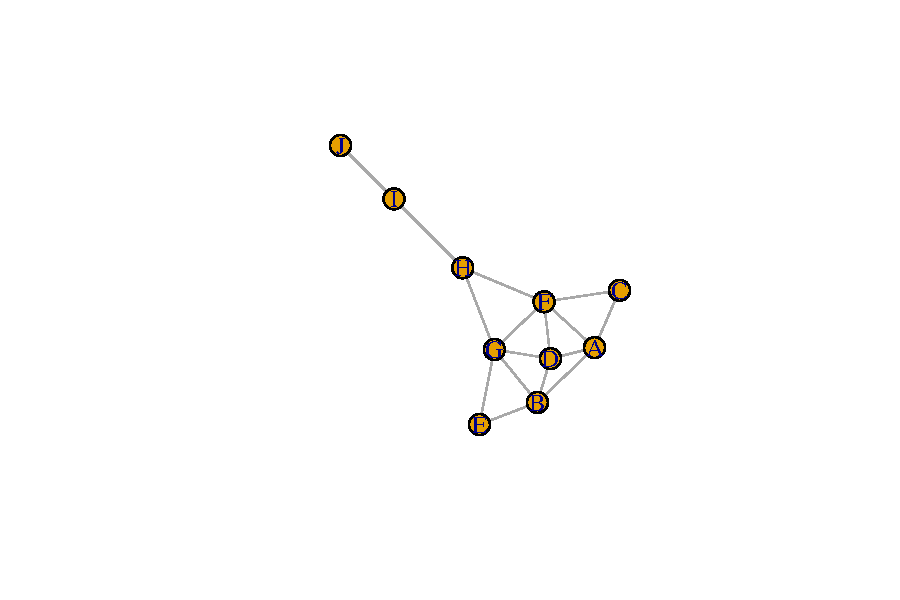
\includegraphics[width=0.25\textwidth]{FIGS/L15-plot-union-graphs-net1-1.pdf}
$\bigcup$
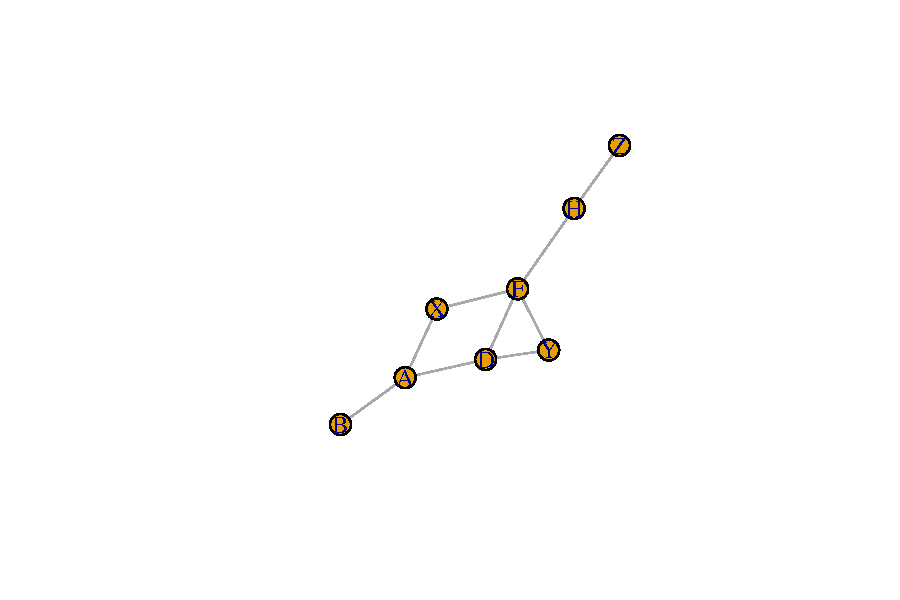
\includegraphics[width=0.25\textwidth]{FIGS/L15-plot-union-graphs-net2-1.pdf}
$\implies$
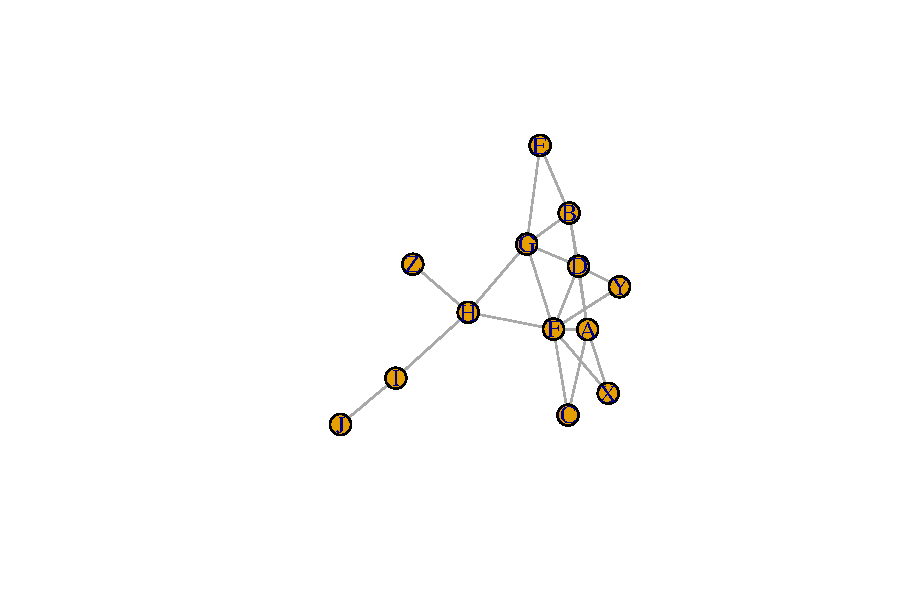
\includegraphics[width=0.3\textwidth]{FIGS/L15-plot-union-graphs-net1Unet2-1.pdf}
\end{frame}

\begin{frame}[fragile]\frametitle{Intersection of two graphs}
\begin{knitrout}
\definecolor{shadecolor}{rgb}{0.969, 0.969, 0.969}\color{fgcolor}\begin{kframe}
\begin{alltt}
\hldef{G_inter} \hlkwb{=} \hldef{net1} \hlopt \hldef{net2}
\hlkwd{plot}\hldef{(G_inter)}
\end{alltt}
\end{kframe}
\end{knitrout}
\end{frame}

\begin{frame}
\centering
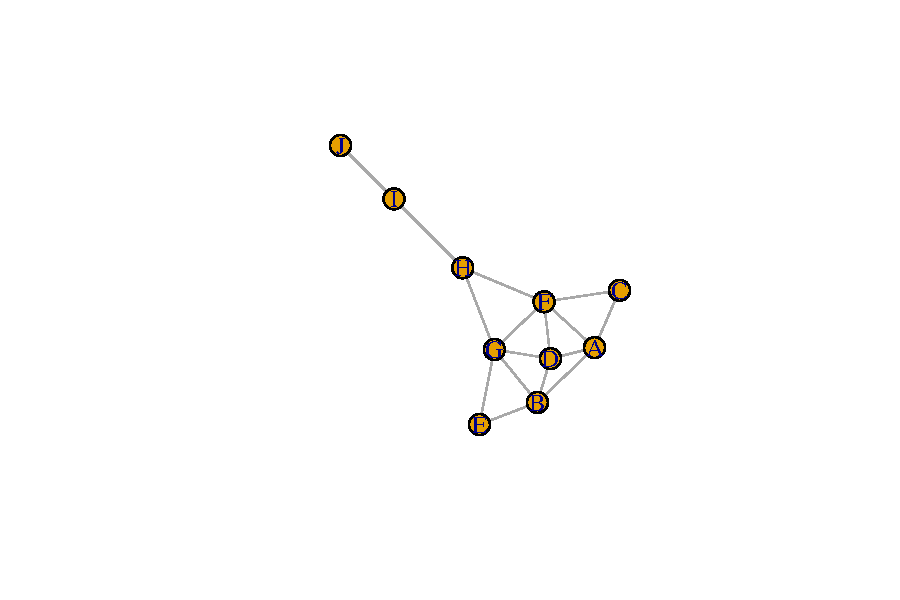
\includegraphics[width=0.25\textwidth]{FIGS/L15-plot-union-graphs-net1-1.pdf}
$\bigcap$
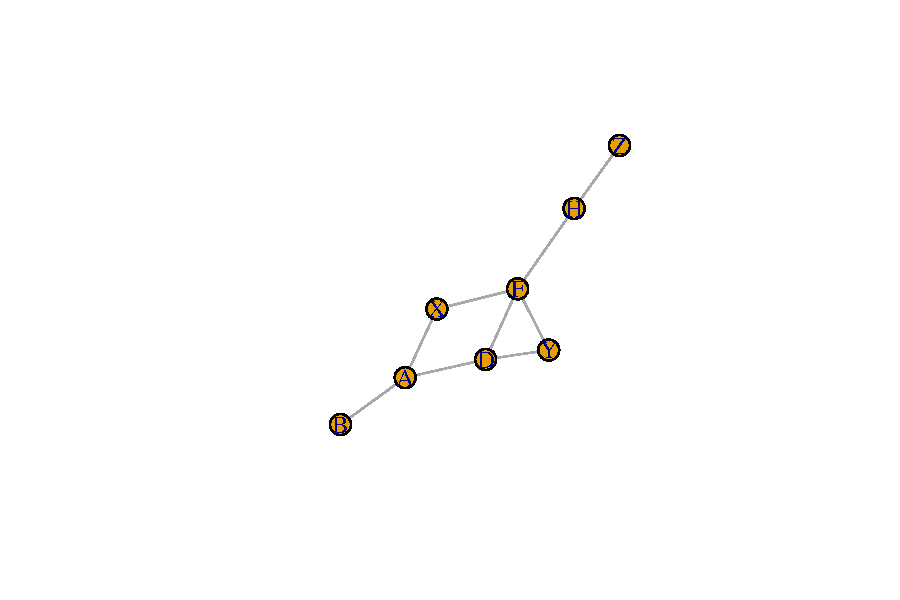
\includegraphics[width=0.25\textwidth]{FIGS/L15-plot-union-graphs-net2-1.pdf}
$\implies$
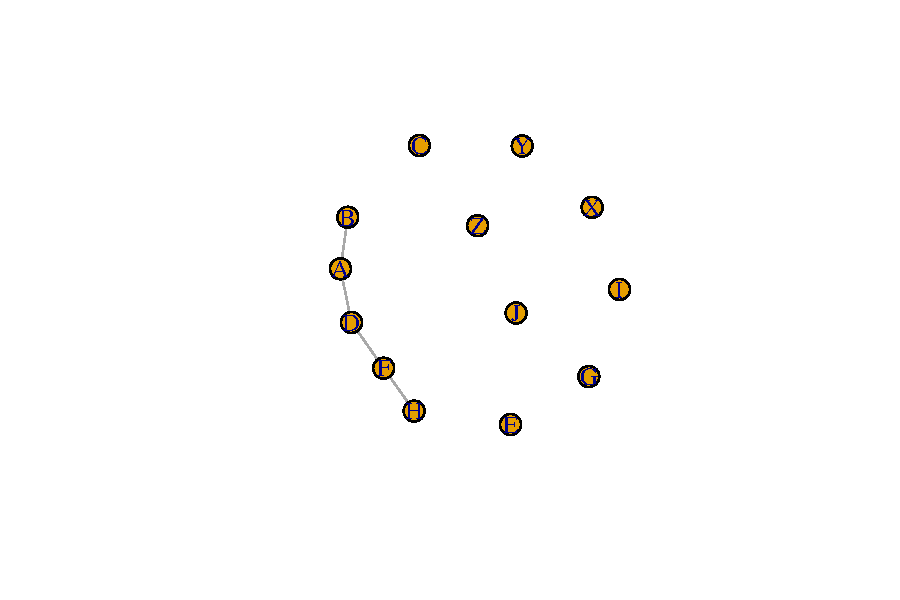
\includegraphics[width=0.3\textwidth]{FIGS/L15-plot-intersection-graphs-net1Nnet2-1.pdf}
\end{frame}



%%%%%%%%%%%%%%%%%%%%%%%%
%%%%%%%%%%%%%%%%%%%%%%%%
%%%%%%%%%%%%%%%%%%%%%%%%
%%%%%%%%%%%%%%%%%%%%%%%%
% \section{Index of terms used}
% \begin{frame}{Index}
% 	\printindex
% \end{frame}

\end{document}
